\chapter{Release 1 Prédiction}
\section*{Introduction}
Une release est constituée d’une suite d’itérations (sprint) qui se terminent quand les incréments de ces derniers
construisent un produit d'une valeur suffisante pour les utilisateurs finaux.\\
La période des releases est définie par le Product Owner en coopération avec son équipe Scrum.
Notre première release sera composée de deux sprints, dont chacun, ayant une vélocité de 28 jours.
Dans ce chapitre, nous allons traiter les "user story" de nos sprints pour produire un produit
potentiellement livrable.
\section{Sprint 1 Création d'un modèle de prédiction}
Le sprint est le coeur de Scrum. Il s’agit d’un bloc de temps pendant lequel un incrément du produit est effectué. Tous les sprints d’une release ont une durée constante et ne se chevauchent
jamais, c’est-à-dire qu’un sprint ne peut pas commencer tant que le précédent n’est pas encore terminé.
Avant de se lancer dans un sprint, l’équipe Scrum doit obligatoirement définir le but de ce dernier qui est défini en terme métier et non pas en terme technique pour qu’il soit compréhensible par les membres en dehors de l’équipe \cite{sprint}.

\subsection{Backlog du Sprint}
Le Backlog du sprint contient une liste des tâches identifiées par l'équipe Scrum qui devront être réalisées avant la fin de sprint.\\

\captionof{table}{Backlog du Sprint 1}

\begin{tabular}{@{}| >{\centering\arraybackslash}p{.04\textwidth}| >{\centering\arraybackslash}p{.30\textwidth}|>{\centering\arraybackslash}p{.06\textwidth}| >{\centering\arraybackslash}p{.35\textwidth}| >{\centering\arraybackslash}p{.13\textwidth}|@{}}

\hline \rowcolor{lightgray} \textbf{ID}  &  \textbf { User Story} & \textbf {ID Tâche} & \textbf {Tâche} & \textbf{Estimation (jours)} \\



\hline

\multirow{4}{*}{1} & \multirow{4}{.30\textwidth}{En tant qu’administrateur, je veux
importer un fichier contenant toutes
les informations des employés.}  & 1.1 
  & Installer les différents packages nécessaires de python et Tensorflow. & 1 \\ 
\cline{3-5}
& &  1.2 & Développer et tester un service web d'import. & 1 \\
\cline{3-5}
& &  1.3 & Mettre en place l’interface d'import. & 1 \\


\hline


\hline
\end{tabular}


%2ème Tabular 

\begin{tabular}{@{}| >{\centering\arraybackslash}p{.04\textwidth}| >{\centering\arraybackslash}p{.30\textwidth}|>{\centering\arraybackslash}p{.06\textwidth}| >{\centering\arraybackslash}p{.35\textwidth}| >{\centering\arraybackslash}p{.13\textwidth}|@{}}

\hline \rowcolor{lightgray} \textbf{ID}  &  \textbf { User Story} & \textbf {ID Tâche} & \textbf {Tâche} & \textbf{Estimation (jours)} \\



\hline

\multirow{4}{*}{2} & \multirow{4}{.30\textwidth}{En tant qu’administrateur, je veux
préparer mes données.}  & 2.1 
  & Éliminer les lignes vides du fichier qui a été importé. & 2 \\ 
\cline{3-5}
& &  2.2 &  Développer et tester un service web qui permet de convertir toutes les données en données numériques et les mettre à la même échelle. & 5\\

\cline{3-5}
& &  2.3 &  Implémenter et tester un service web qui permet de diviser les données en des données d'apprentissage pour créer notre modèle et des données de test pour évaluer notre modèle construit. & 1\\
\hline


%Third row in table 2
\multirow{4}{*}{3} & \multirow{4}{.30\textwidth}{En tant qu’administrateur, je veux
construire un modèle de prédiction.}  & 3.1 
  & Évaluer et adapter nos données aux différentes solutions existantes pour créer notre modèle de prédiction. & 2 \\ 
\cline{3-5}
& &  3.2 &  Construire un algorithme basé sur le réseau de neurones comme étant notre modèle de prédiction vu sa grande performance et l'exposer sous format de service web. & 6\\


\hline

%4th row in table 2
\multirow{4}{*}{4} & \multirow{4}{.30\textwidth}{En tant qu’administrateur, je
souhaite évaluer mon modèle.}  & 4.1 
  &  Développer et tester un service web qui permet d'évaluer et tester la performance de notre modèle de prédiction avec les données de test. & 6 \\ 
\hline




\hline
\end{tabular}


\begin{tabular}{@{}| >{\centering\arraybackslash}p{.04\textwidth}| >{\centering\arraybackslash}p{.30\textwidth}|>{\centering\arraybackslash}p{.06\textwidth}| >{\centering\arraybackslash}p{.35\textwidth}| >{\centering\arraybackslash}p{.13\textwidth}|@{}}

\hline \rowcolor{lightgray} \textbf{ID}  &  \textbf { User Story} & \textbf {ID Tâche} & \textbf {Tâche} & \textbf{Estimation (jours)} \\



\hline

%1th row in table 3
\multirow{4}{*}{5} & \multirow{5}{.30\textwidth}{En tant qu’utilisateur, je veux
effectuer des prédictions sur la
démission des employés.}  & 5.1 
  &  Développer et tester un service web qui permet d'effectuer des prédictions. & 1 \\ 
  \cline{3-5}
& &  5.2 &  Mettre en place l’interface de prédiction. & 1\\
\hline


\hline
\end{tabular}



\subsection{Spécification fonctionnelle}
La figure \ref{fig:usecaseModel} illustre le diagramme de cas d’utilisation détaillé de «Créer un modèle de prédiction».
    \begin{figure}[htpb]
    \centering
    \fcolorbox{brown}{white}{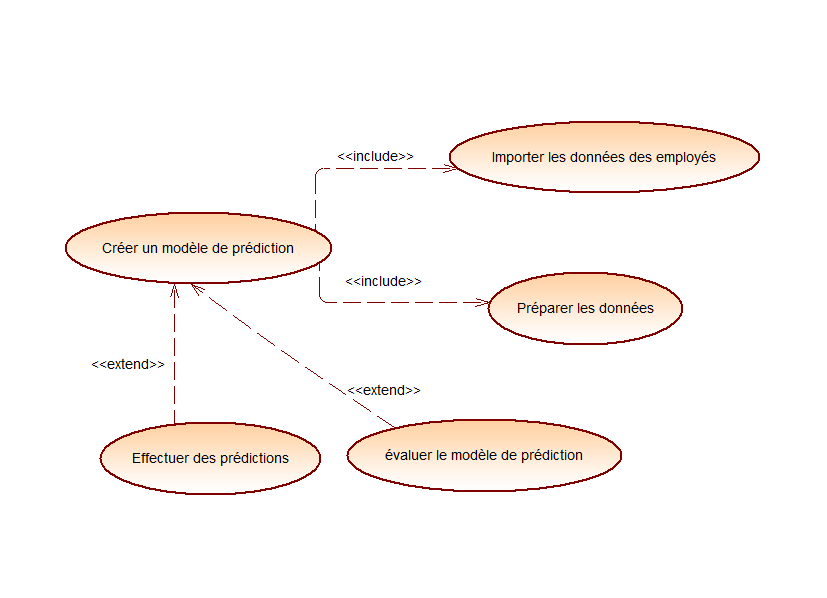
\includegraphics[width=1\linewidth]{img/sprint1_usecase.png}}
    \caption{Diagramme de cas d’utilisation « Créer un modèle de prédiction »}
    \label{fig:usecaseModel}
    \end{figure}
\newpage

Le tableau \ref{tab:importData} présente la description textuelle du cas d’utilisation « Importer les données des employés ».
\begin{longtable}[c]{
    |p{.35\textwidth}
    |p{.61\textwidth}|
}
    \caption{Description du diagramme de cas d’utilisation <<Importer les données des employés>>}
    \label{tab:importData}\\
    \hline
    
    Cas d’utilisation
    & Importer les données des employés. \\
    \hline 
    
    Acteur
    & Administrateur. \\
    \hline 
    
    Précondition
    & Les données doivent être sous format <<csv>>. \\
    \hline
    
    Post-condition
    & Données importées. \\
    \hline
    
    Description du
scénario

    &     \begin{itemize}
    \item L’administrateur accède à l'interface d'import.
    \item L’administrateur sélectionne  un fichier contenant les informations des employés.
    \end{itemize} \\
    \hline
    
   Exception
    & Erreur de format de fichier ou de connexion.
 \\ \hline
   
\end{longtable}




Le tableau \ref{tab:modèle} présente la description textuelle du cas d’utilisation « Construire un modèle de prédiction ».
\begin{longtable}[c]{
    |p{.35\textwidth}
    |p{.61\textwidth}|
}
    \caption{Description du diagramme de cas d’utilisation <<Construire un modèle de prédiction>>}
    \label{tab:modèle}\\
    \hline
    
    Cas d’utilisation
    & Construire un modèle de prédiction. \\
    \hline 
    
    Acteur
    & Administrateur. \\
    \hline 
    
    Précondition
    & Les données pour l'apprentissage et pour le test existent. \\
    \hline
    
    Post-condition
    & Modèle construit. \\
    \hline
    
    Description du
scénario

    &     \begin{itemize}
    \item L’administrateur appel le service web de création du modèle.
    \end{itemize} \\
    \hline
    
   Exception
    & Erreur de format de données ou de connexion.
 \\ \hline
   
\end{longtable}



\newpage
Le tableau \ref{tab:EvaluationModèle} présente la description textuelle du cas d’utilisation «Évaluer le modèle de prédiction».
\begin{longtable}[c]{
    |p{.35\textwidth}
    |p{.61\textwidth}|
}
    \caption{Description du diagramme de cas d’utilisation <<Évaluer le modèle de prédiction>>}
    \label{tab:EvaluationModèle}\\
    \hline
    
    Cas d’utilisation
    & Évaluer le modèle de prédiction. \\
    \hline 
    
    Acteur
    & Administrateur. \\
    \hline 
    
    Précondition
    & Le modèle doit être créé. \\
    \hline
    
    Post-condition
    & Modèle évalué. \\
    \hline
    
    Description du
scénario

    &     \begin{itemize}
    \item L’administrateur appelle le service web qui permet d'évaluer le modèle de prédiction .
    \end{itemize} \\
    \hline
    
   Exception
    & Erreur  de connexion.
 \\ \hline
   
\end{longtable}


Le tableau \ref{tab:effectuer_prediction} présente la description textuelle du cas d’utilisation « Effectuer des prédictions ».
\begin{longtable}[c]{
    |p{.35\textwidth}
    |p{.61\textwidth}|
}
    \caption{Description du diagramme de cas d’utilisation << Effectuer des prédictions >>}
    \label{tab:effectuer_prediction}\\
    \hline
    
    Cas d’utilisation
    & Effectuer des prédictions. \\
    \hline 
    
    Acteur
    & Administrateur. \\
    \hline 
    
    Précondition
    & Le modèle doit être créé. \\
    \hline
    
    Post-condition
    & Prédiction effectuée. \\
    \hline
    
    Description du
scénario

    &     \begin{itemize}

    \item L’administrateur effectue des prédictions sur la démission des employés.
    \end{itemize} \\
    \hline
    
   Exception
    & Erreur de format de données ou de connexion.
 \\ \hline
   
\end{longtable}












\subsection{Apprentissage Automatique}
Dans cette partie, nous allons construire notre modèle de prédiction qui est basé sur l'apprentissage automatique ou Machine learning en anglais.
En effet, l'apprentissage automatique est défini comme étant un champ d’étude qui donne aux ordinateurs la capacité d’apprendre sans être explicitement programmés. Pour être plus clair, ce que fait le machine learning, c’est apprendre à résoudre un problème de manière automatique en utilisant les données. Dans le cadre du traitement de la donnée, il s’agit de construire un modèle obtenu directement à partir d’exemples. L’objectif des algorithmes de machine learning est de minimiser ce qu’on appelle l’erreur, c’est-à-dire de se tromper le moins possible \cite{MachineLearning}.

Nous distinguons différents types d'apprentissage automatique dont les plus connus sont les suivants :
   \subsubsection{Apprentissage Automatique supervisé}
  Récupération des données annotées à partir de leurs sorties pour entraîner le modèle, c'est-à-dire une classe cible ou une étiquette qui leur a déjà été attribuée et nous voulons que l'algorithme devienne capable de le prédire sur de nouvelles données non annotées une fois entraînées.\\
  La figure \ref{fig:usecaseMLSupervised} décrit les différentes étapes de l'apprentissage automatique supervisé.
  \vspace{0.25cm}
      \begin{figure}[htpb]
    \centering
    \fcolorbox{brown}{white}{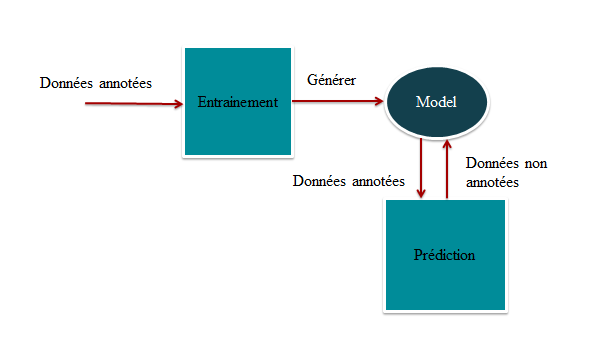
\includegraphics[width=1\linewidth]{img/ApprentissageSupervise2.png}}
    \caption{Apprentissage Automatique supervisé}
    \label{fig:usecaseMLSupervised}
    \end{figure}

    \subsubsection{Apprentissage Automatique non supervisé}
    Les données d'entrées ne sont pas annotées. L'algorithme d'entraînement s'applique dans ce cas à trouver seul les similarités et distinctions au sein de ces données et à regrouper ensemble celles qui partagent des caractéristiques communes.

    La principale différence lorsque nous parlons d'apprentissage non supervisé est que nous n'avons plus d'exemples. Il n'est donc plus possible d'évaluer la performance de l'algorithme en comparant le résultat avec les valeurs observées. Les problèmes d'apprentissage non supervisé les plus populaires sont les analyses de regroupement \cite{unSupervised}.
\subsection{Solutions existantes}
La phase la plus importante dans l'apprentissage automatique, c'est d'identifier de quel type d'apprentissage nous allons utiliser pour répondre à notre problème.\\
La figure \ref{fig:usecasedata} expose la structure de nos données.
 \begin{figure}[htpb]
    \centering
    \fcolorbox{brown}{white}{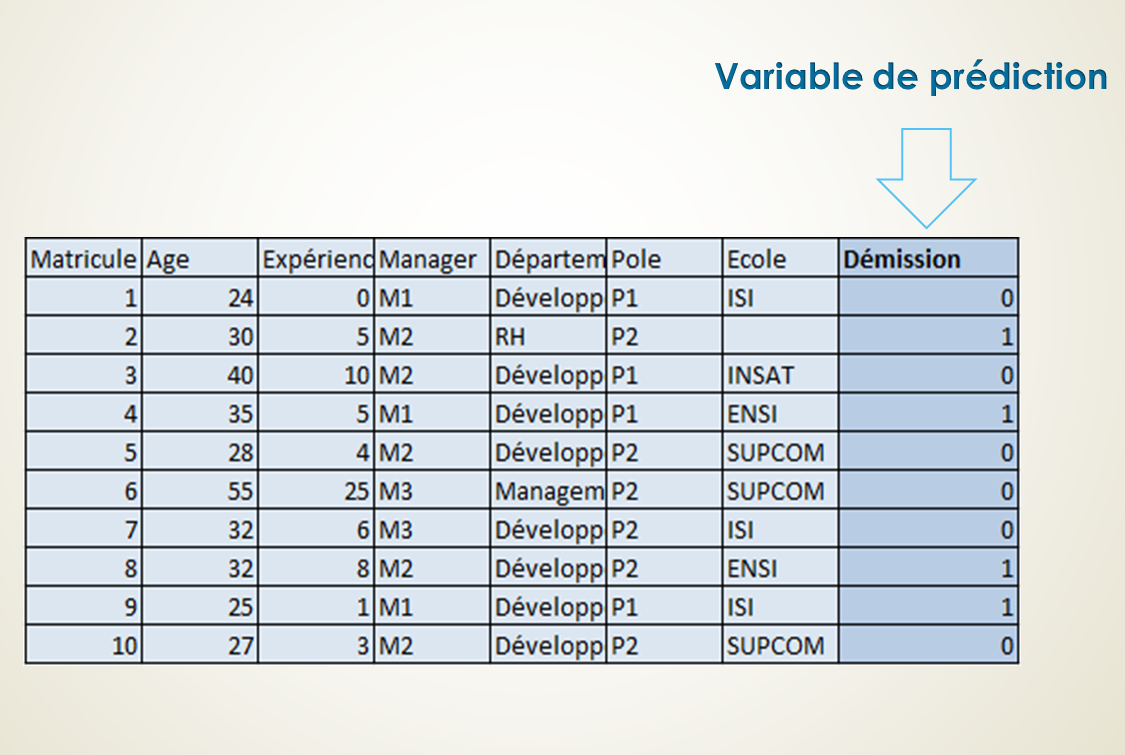
\includegraphics[width=1\linewidth]{img/data.png}}
    \caption{Structure de nos données}
    \label{fig:usecasedata}
    \end{figure}
    \\
Cette structure est une représentation de nos données contenues dans  un fichier excel comportant toutes les informations des employés de la société.
Nos données sont annotées et nous avons pour chaque donnée sa sortie (label, étiquette) qui est démission considérée comme étant une variable de prédiction ( « 1 » : l'employé va démissionner,   « 0 » : l’employé va rester dans Sofrecom  ).\\
Notre choix s'est porté sur l'apprentissage supervisé vu que toutes nos données sont étiquetées et nous allons utiliser les différents algorithmes de cet apprentissage pour construire notre modèle de prédiction.
    \subsubsection{Classification}
    C’est lorsque le type de sortie que le nous attendons de notre programme est une valeur discrète (une catégorie). Dans notre cas, nous avons deux classes pour la démission (0 ou 1 ).\\
    Nous avons appliqué plusieurs algorithmes de classification sur nos données et nous allons évaluer chaque modèle avec la matrice de confusion comme le montre la figure \ref{fig:ConfusionMatrix}.
     \begin{figure}[htpb]
    \centering
    \fcolorbox{brown}{white}{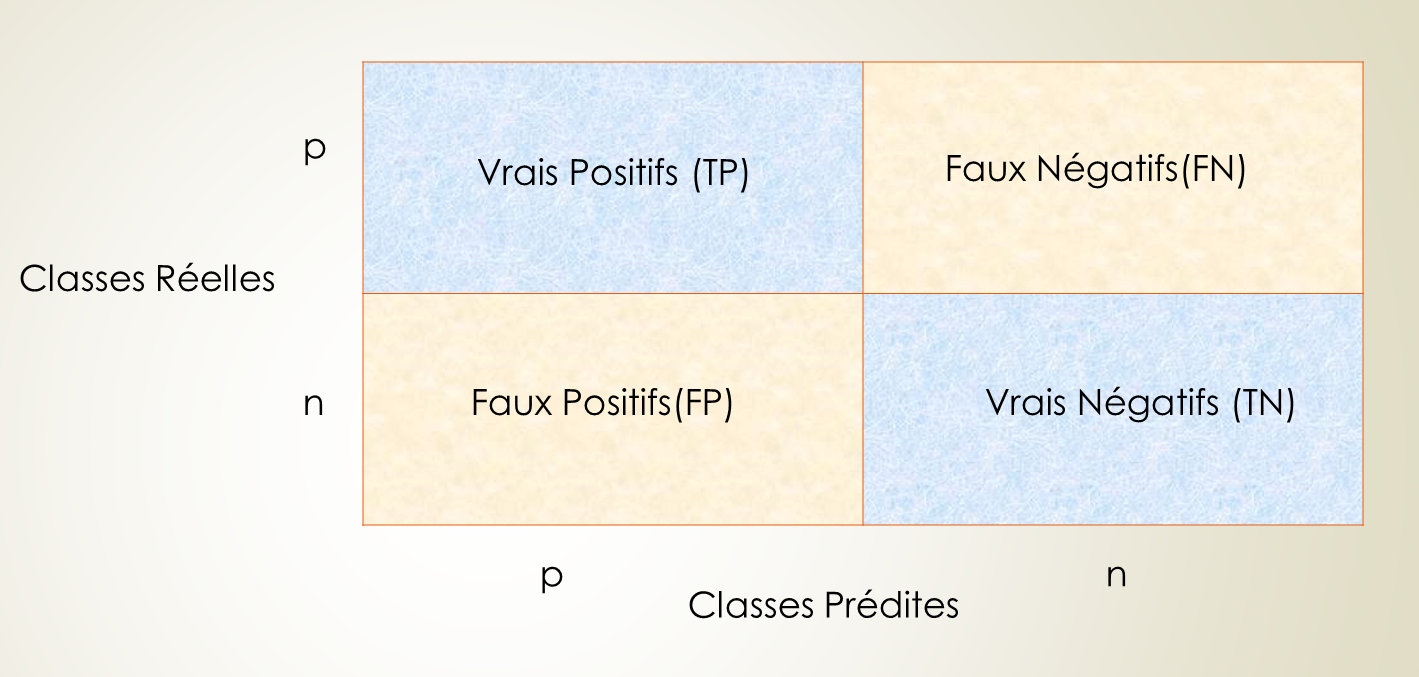
\includegraphics[width=1\linewidth]{img/confusion2.png}}
    \caption{Matrice de confusion}
    \label{fig:ConfusionMatrix}
    \end{figure}
    \\
    Nous allons définir chaque notion présentée dans la figure \ref{fig:ConfusionMatrix} :
    \begin{itemize}
        \item TP (Vrais positifs) : Mesure la proportion de positifs correctement identifiés comme tels;
        \item TN (Vrais négatifs) : Mesure la proportion de négatifs qui sont correctement identifiés comme tels;
        \item FP (Faux positifs) : Est un résultat qui indique qu’une condition donnée a été remplie, quand ce n’est pas le cas. C’est à dire, par erreur, un effet positif a été supposé;
        \item FN (Faux négatifs) : Est lorsqu'un un résultat de test indique qu’une condition a échoué, alors qu’elle était réussie.

 \end{itemize}
\textbf{Machine à Vecteurs de Support ( SVM )} \\
C'est un algorithme de classification binaire qui a pour objectif de trouver la séparation entre deux classes d’objets avec l’idée que plus la séparation est large, plus la classification est robuste  \cite{SVM}.
   Nous avons appliqué le modèle SVM sur nos données et nous avons obtenu comme résultats suivants concernant la performance de ce modèle comme le montre la figure \ref{fig:confusionMatrixSVM}.
     \begin{figure}[htpb]
    \centering
    \fcolorbox{brown}{white}{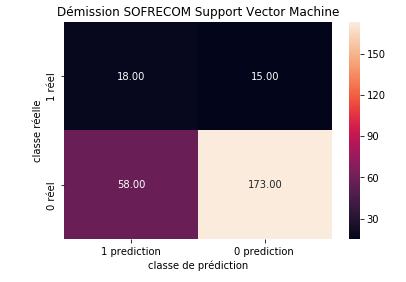
\includegraphics[width=0.8\linewidth]{img/SVM.png}}
    \caption{Matrice de confusion de SVM}
    \label{fig:confusionMatrixSVM}
    \end{figure}
    \\
Ce modèle contient 73 erreurs sur 264 données et il contient un taux de précision de 0.69 comme le montre la figure \ref{fig:ConfusionMatrixSVMPrecision}.\\
   \begin{figure}[htpb]
    \centering
    \fcolorbox{brown}{white}{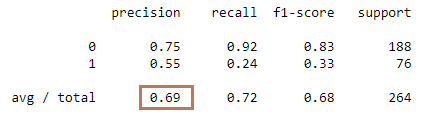
\includegraphics[width=0.8\linewidth]{img/svmprecision.png}}
    \caption{Précision du modèle SVM}
    \label{fig:ConfusionMatrixSVMPrecision}
    \end{figure}
    \\
    \textbf{NB : }La précision est la fraction des instances pertinentes parmi les instances récupérées. Elle est calculée à l’aide de la formule suivante :
\[Precision=\frac{\sum{TP}}{\sum{(TP + FP)}}\]
    Ce modèle ne permet pas de donner la valeur de la prédiction sous un format de probabilité (pourcentage). De plus, le taux d’erreur est très grand.
    \newpage
    
\textbf{Arbre de décision} \\    
Les arbres de décision sont l’une des structures de données majeures de l’apprentissage statistique. Leur fonctionnement repose sur des heuristiques qui, tout en satisfaisant l’intuition, donnent des résultats remarquables \cite{DecisonTree}.
  Nous avons appliqué le modèle arbre de décision sur nos données et nous avons obtenu comme résultats suivants concernant la performance de ce modèle comme le montre la figure \ref{fig:ConfusionMatrixDecsionTree}.

     \begin{figure}[htpb]
    \centering
    \fcolorbox{brown}{white}{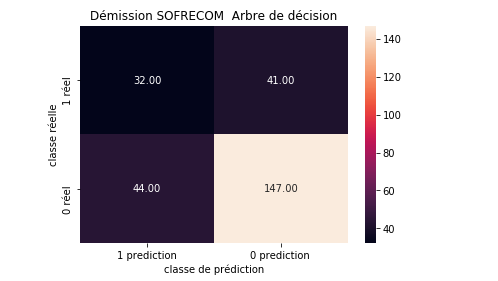
\includegraphics[width=0.8\linewidth]{img/decisionTree.png}}
    \caption{Matrice de confusion d'arbre de décision}
    \label{fig:ConfusionMatrixDecsionTree}
    \end{figure}
    
Ce modèle contient 85 erreurs sur 264 données et il contient un taux de précision de 0.67 comme le montre la figure     \ref{fig:ConfusionMatrixDecisionTreePrecision}.
   \begin{figure}[htpb]
    \centering
    \fcolorbox{brown}{white}{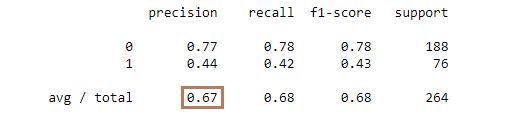
\includegraphics[width=0.8\linewidth]{img/DecisionTreePrecision.png}}
    \caption{Précision du modèle d'arbre de décision}
    \label{fig:ConfusionMatrixDecisionTreePrecision}
    \end{figure}

    Ce modèle ne permet pas de donner la valeur de la prédiction sous un format de probabilité (pourcentage). De plus, le taux d’erreur est très grand.

\newpage

\textbf{Forêt d'arbres décisionnels ( Random Forest )} \\
L'algorithme des forêts d'arbres décisionnels effectue un apprentissage sur de multiples arbres de décision entraînés sur des sous-ensembles de données légèrement différents \cite{RandomForest}.\\
   Nous avons appliqué le modèle forêt d'arbres décisionnels sur nos données et nous avons obtenu comme résultats suivants concernant la performance de ce modèle comme le montre la figure \ref{fig:ConfusionRandomForest}.
     \begin{figure}[htpb]
    \centering
    \fcolorbox{brown}{white}{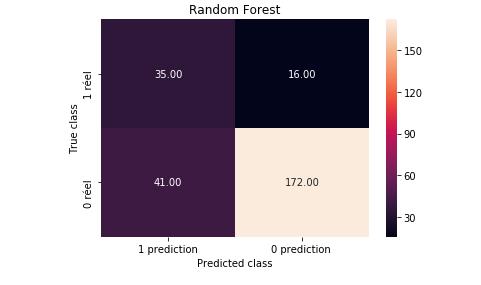
\includegraphics[width=0.8\linewidth]{img/RandomForest.png}}
    \caption{Matrice de confusion de forêt d'arbres décisionnels}
    \label{fig:ConfusionRandomForest}
    \end{figure}
    \\
Ce modèle contient 57 erreurs sur 264 données et il contient un taux de précision de 0.77 comme le montre la figure \ref{fig:ConfusionMatrixRandomForestPrecisionss}.
   \begin{figure}[htpb]
    \centering
    \fcolorbox{brown}{white}{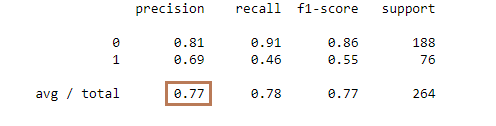
\includegraphics[width=0.8\linewidth]{img/RandomForestPrecision.png}}
    \caption{Précision du modèle de forêt d'arbres décisionnels}
    \label{fig:ConfusionMatrixRandomForestPrecisionss}
    \end{figure}
    \\
    Ce modèle ne permet pas de donner la valeur de la prédiction sous un format de probabilité (pourcentage). De plus, le taux d’erreur est très grand.
    \newpage
    

\textbf{K plus proches voisins (K-Nearest Neighbors ou KNN)} \\
C'est une méthode d’apprentissage supervisé. Il existe une base de données d'apprentissage composée de N paires "entrées-sorties". Pour estimer la sortie associée à une nouvelle entrée x, la méthode des k plus proches voisins consiste à prendre en compte (de manière identique) les k échantillons d'apprentissage dont l'entrée est la plus proche de la nouvelle entrée x \cite{KNN}.\\
   Nous avons appliqué le modèle KNN sur nos données et nous avons obtenu comme résultats suivants concernant la performance de ce modèle comme le montre la figure \ref{fig:ConfusionKNN}.
     \begin{figure}[htpb]
    \centering
    \fcolorbox{brown}{white}{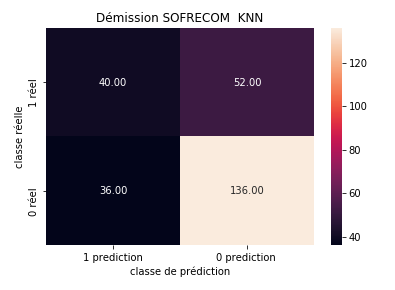
\includegraphics[width=0.8\linewidth]{img/KNN.png}}
    \caption{Matrice de confusion de KNN}
    \label{fig:ConfusionKNN}
    \end{figure}
    \\
Ce modèle contient 88 erreurs sur 264 données et il contient un taux de précision de 0.69 comme le montre la figure \ref{fig:ConfusionMatrixKNNPrecision}.
   \begin{figure}[htpb]
    \centering
    \fcolorbox{brown}{white}{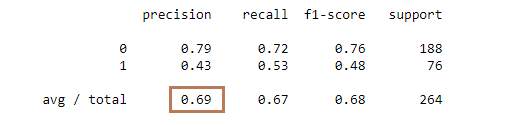
\includegraphics[width=0.8\linewidth]{img/KNNPrecision.png}}
    \caption{Précision du modèle de KNN}
    \label{fig:ConfusionMatrixKNNPrecision}
    \end{figure}
    \\
    Ce modèle ne permet pas de donner la valeur de la prédiction sous un format de probabilité (pourcentage). De plus, le taux d’erreur est très grand.
    \newpage
    


%Gradient boosting Classifier
\textbf{Gradient Boosting Classifier} \\
Le gradient boosting est une technique d'apprentissage machine pour les problèmes de régression et de classification, qui produit un modèle de prédiction sous la forme d'un ensemble de modèles de prédiction faibles, généralement des arbres de décision. Il construit le modèle par étapes, comme les autres méthodes de boosting, et il les généralise en permettant l'optimisation d'une fonction de perte arbitraire différentiable \cite{GradientBoostingClassifier}.\\
   Nous avons appliqué le modèle KNN sur nos données et nous avons obtenu comme résultats suivants concernant la performance de ce modèle comme le montre la figure \ref{fig:ConfusionGRadientBoostingClassifier}.
     \begin{figure}[htpb]
    \centering
    \fcolorbox{brown}{white}{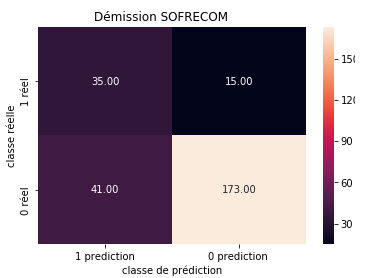
\includegraphics[width=0.75\linewidth]{img/GRadientBoostingClassifier2.png}}
    \caption{Matrice de confusion de Gradient Boosting Classifier}
    \label{fig:ConfusionGRadientBoostingClassifier}
    \end{figure}
    \\
Ce modèle contient 56 erreurs sur 264 données et il contient un taux de précision de 0.78 comme le montre la figure     \ref{fig:ConfusionMatrixGRadientBoostingClassifierPrecision}.
   \begin{figure}[htpb]
    \centering
    \fcolorbox{brown}{white}{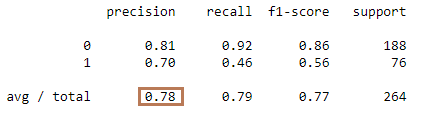
\includegraphics[width=0.75\linewidth]{img/GRadientBoostingClassifierPrecision.png}}
    \caption{Précision du modèle de Gradient Boosting Classifier}
    \label{fig:ConfusionMatrixGRadientBoostingClassifierPrecision}
    \end{figure}
    \\
    Ce modèle ne permet pas de donner la valeur de la prédiction sous un format de probabilité (pourcentage). De plus, le taux d’erreur est très grand.
    \newpage
    



\newpage
    \subsubsection{Régression}
    C’est lorsque le type de sortie que le nous attendons de notre programme est une valeur continue ou quantitative \cite{RegressionGloabal}.\\
    Dans cette partie, nous allons aborder les différents algorithmes de régression sur nos données.
\textbf{Régression linéaire} \\
C'est un modèle qui cherche à établir une relation linéaire entre une variable, dite expliquée, et une ou plusieurs variables, dites explicatives.
\[Y= w1*x1 + w2*x2 + w3*x3 + … + wn*xn + b\]
\begin{itemize}
    \item Y : variable dépendante (expliquée);
    \item xi : variable indépendante (explicative);
    \item b : ordonnée à l’origine (biais);
    \item wi : poid/pente (variation moyenne de la valeur d'Y par rapport à xi).
\end{itemize}

Dans notre cas, nous avons la démission comme variable expliquée et comme variables explicatives ( civilité, expérience avant sofrecom, expérience sofrecom, expérience totale, séniorité, niveau académique, poste, pôle, manager, âge, situation familiale ).\\
Nous avons appliqué le modèle régression linéaire sur nos données et nous avons testé sur 20 données comme le montre la figure     \ref{fig:LinearRegression}.

   \begin{figure}[htpb]
    \centering
    \fcolorbox{brown}{white}{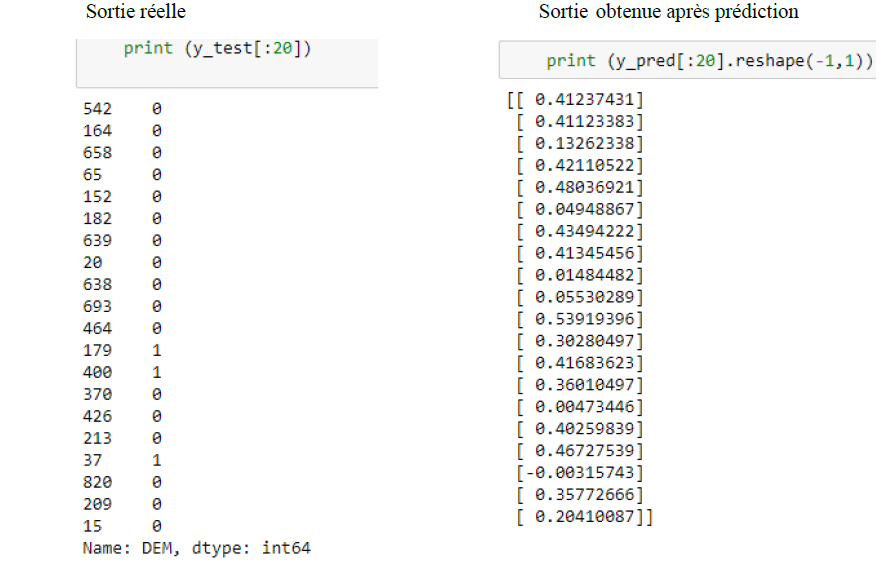
\includegraphics[width=0.63\linewidth]{img/linearRegressionTest.png}}
    \caption{Test sur le modèle de régression linéaire}
    \label{fig:LinearRegression}
    \end{figure}
Comme le montre la figure \ref{fig:LinearRegression}, le modèle construit n'est pas performant et n'est pas adapté à notre problème.
\newpage
\textbf{Gradient Boosting Regressor} \\
De même pour l'algorithme de Gradient Boosting Regressor, le modèle appliqué sur nos données n'est pas adapté à notre problème comme le montre la figure     \ref{fig:GBR}.
   \begin{figure}[htpb]
    \centering
    \fcolorbox{brown}{white}{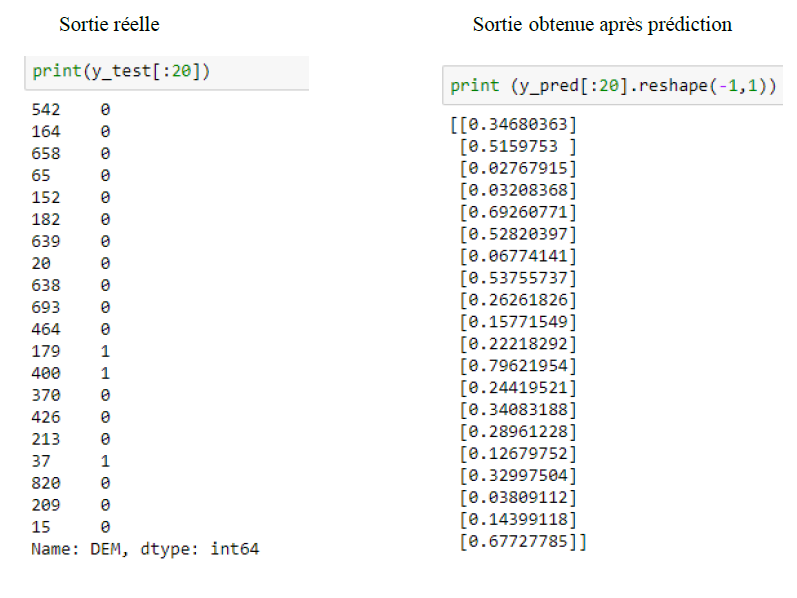
\includegraphics[width=0.68\linewidth]{img/GBR.png}}
    \caption{Test sur le modèle de Gradient Boosting Regressor}
    \label{fig:GBR}
    \end{figure}
    
\textbf{Forêt d'arbres décisionnels de régression ( Random Forest Regressor )} \\
De manière similaire pour l'algorithme de forêt d'arbres décisionnels de régression, le modèle appliqué sur nos données n'est pas adapté à notre problème comme le montre la figure   \ref{fig:RDR}.
   \begin{figure}[htpb]
    \centering
    \fcolorbox{brown}{white}{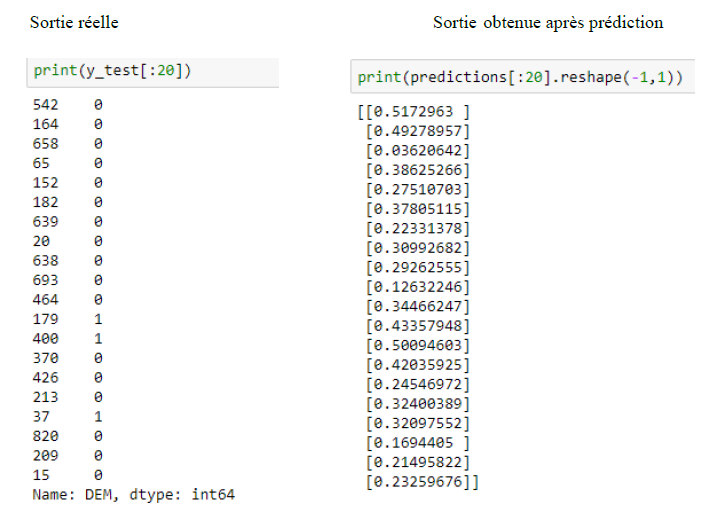
\includegraphics[width=0.68\linewidth]{img/RFR.png}}
    \caption{Test sur le modèle de forêt d'arbres décisionnels de régression }
    \label{fig:RDR}
    \end{figure}

\newpage
\textbf{Gradient Boosting Machine ( GBM ) de H2O Flow} \\
C'est avec cet algorithme que sofrecom construit le modèle de prédiction sur la démission de ses employés. Avec cet algorithme, nous avons créé un nouveau modèle avec nos nouvelles données actualisées comme le montre la figure     \ref{fig:GBM1}. 
   \begin{figure}[htpb]
    \centering
    \fcolorbox{brown}{white}{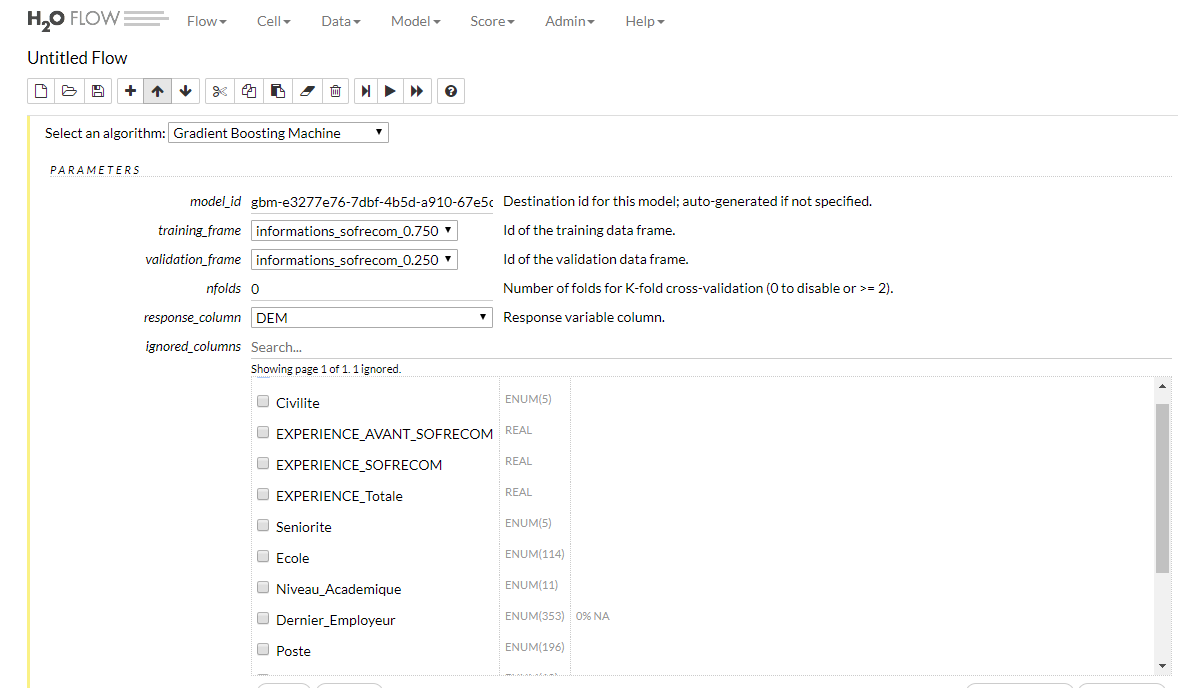
\includegraphics[width=0.62\linewidth]{img/gbm1.png}}
    \caption{Création du modèle GBM avec H2O Flow}
    \label{fig:GBM1}
    \end{figure} \\
Nous avons construit notre modèle avec les données d'apprentissage (75\% de totalité nos données) et les autres données qui sont les données de test sont utilisées pour l'évaluation de notre modèle.\\
La figure \ref{fig:GBM2} décrit l'évaluation de notre modèle avec l'importance de chaque variable explicative.
   \begin{figure}[htpb]
    \centering
    \fcolorbox{brown}{white}{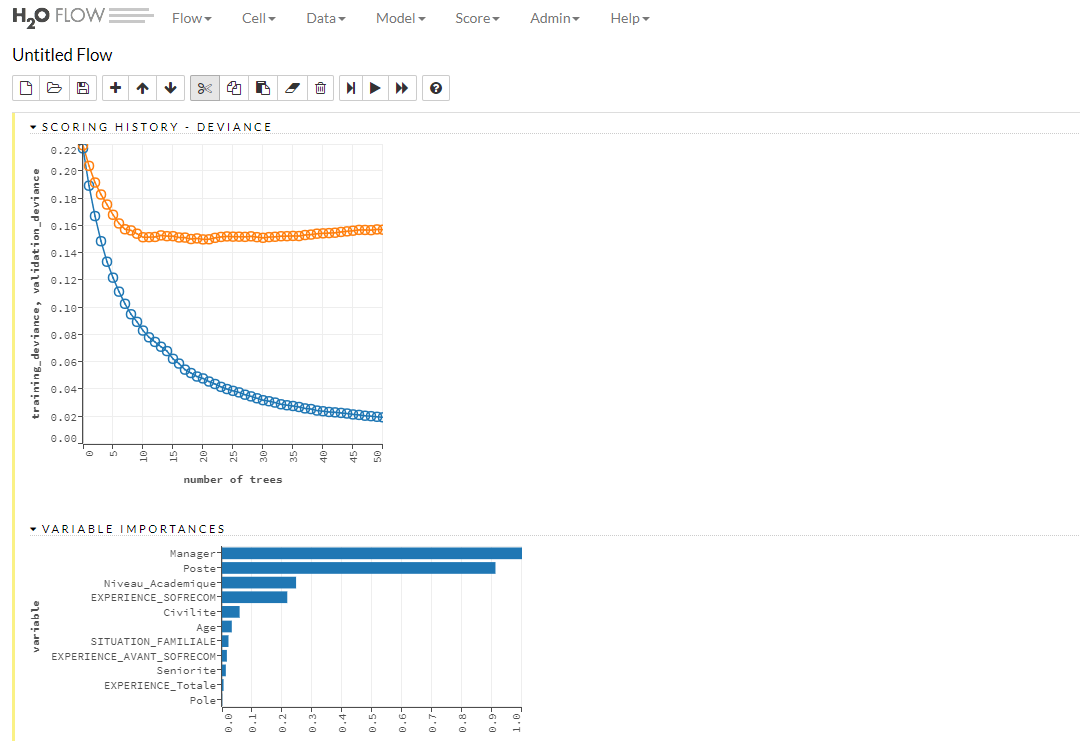
\includegraphics[width=0.62\linewidth]{img/gbm2.png}}
    \caption{Évaluation du GBM et importance de chaque variable explicative}
    \label{fig:GBM2}
    \end{figure}\\
Les deux courbes (données d'apprentissage en bleu et données de test en orange) ne sont pas concordantes, elles sont par contre très éloignées l'une de l'autre ce qui nous indique que ce modèle n'est pas adapté à notre problème.
\newpage
\subsection{Solution envisagée}
Notre solution consiste à aller en profondeur et construire un réseau de neurones qui permet de regrouper plusieurs algorithmes pour pouvoir traiter nos données et avoir un modèle de prédiction performant.
Les algorithmes d'apprentissage en profondeur tentent d'apprendre des fonctionnalités de haut niveau à partir de données. Par conséquent, l'apprentissage en profondeur réduit la tâche de développement d'un nouvel extracteur de caractéristiques pour chaque problème.\\
La différence la plus importante entre l'apprentissage en profondeur et l'apprentissage automatique traditionnel est sa performance à mesurer quand l'échelle des données augmente. 

\subsubsection{Réseau de neurones}
C'est un modèle inspiré du fonctionnement cérébral, qui se compose de couches, dont au moins une est cachée, contenant des unités connectées simples, ou neurones, suivies de non-linéarités.
Les neurones reçoivent plusieurs valeurs d'entrée et génèrent une valeur de sortie. Le neurone calcule la valeur de sortie en appliquant une fonction d'activation (transformation non linéaire) à une somme pondérée des valeurs d'entrée \cite{NeuralNetwork}.\\
Parmi les frameworks les plus connus pour construire un réseau de neurones, nous trouvons Tensorflow. En effet, TensorFlow propose plusieurs Estimators prédéfinis, notamment le plus connu est « DNNRegressor » que nous allons l’utilisé dans notre cas. 
\subsubsection{Préparation des données}
Dans la couche d'entrée de réseau de neurones, les données doivent être des données numériques. Alors, la première phase de préparation des données consiste à convertir les données catégorielles (un ensemble discret de valeurs possibles) en des données numériques et pour ce cas nous allons utiliser la bibliothèque de python « map » comme le montre la figure     \ref{fig:mapPython}.
  \begin{figure}[htpb]
    \centering
    \fcolorbox{brown}{white}{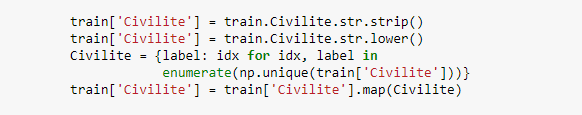
\includegraphics{img/civ0.png}}
    \caption{Script de conversion des données}
    \label{fig:mapPython}
    \end{figure}
    \newpage
Les données sont converties en indexant chaque donnée catégorielle en donnée numérique comme le montre la figure \ref{fig:civilite} pour la variable explicative « civilité ».
  \begin{figure}[htpb]
    \centering
    \fcolorbox{brown}{white}{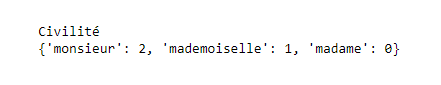
\includegraphics{img/civ2.png}}
    \caption{Exemple de conversion des données}
    \label{fig:civilite}
    \end{figure}
    \\
\textbf{Normalisation des données}\\
La deuxième phase de préparation qui est la normalisation des données consiste à convertir une plage réelle de valeurs en une plage standard de valeurs, généralement de 0 à 1. Supposons que la plage naturelle d'une certaine caractéristique s'étende de 800 à 6 000. En effectuant diverses soustractions et divisions, nous pouvons normaliser ces valeurs à une plage s'étendant de 0 à +1.\\
Dans notre cas, nous allons utiliser la bibliothèque «MinMaxScaler» de la bibliothèque «sklearn.preprocessing» qui est basée sur la formule suivante :
\[X_{norm}=\frac{(X - X_{min})}{(X_{max} - X_{min})}\]
Exemple de nos données traitées après la phase de la normalisation (l’échelle de toutes nos données est devenue entre 0 et 1) comme le montre la figure \ref{fig:normalisedata}.
   \begin{figure}[htpb]
    \centering
    \fcolorbox{brown}{white}{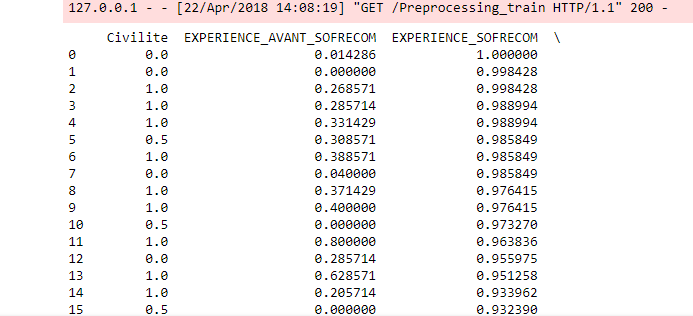
\includegraphics[width=1\linewidth]{img/pre3.png}}
    \caption{données normalisées}
    \label{fig:normalisedata}
    \end{figure}
\newpage
\textbf{Division des données}\\
Cette phase consiste à diviser nos données en des données d'apprentissage pour construire et entraîner notre modèle et des données de test pour évaluer la performance de notre modèle.
Comme le montre la figure \ref{fig:splitdata}, nous avons choisi de diviser nos données en 80\% pour les données d'apprentissage et les autres 20\% pour les données de test.
   \begin{figure}[htpb]
    \centering
    \fcolorbox{brown}{white}{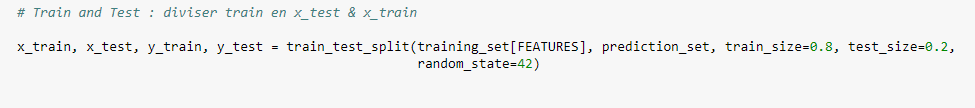
\includegraphics[width=1\linewidth]{img/pre5.png}}
    \caption{données divisées}
    \label{fig:splitdata}
    \end{figure}

\subsubsection{Architecture de réseau de neurones}
Nous allons nous intéresser au perceptron multicouche (architecture de réseau de neurones) qui est organisé en plusieurs couches au sein desquelles une information circule de la couche d'entrée vers la couche de sortie uniquement. Il s'agit donc d'un réseau à propagation directe (feed-forward) qui comporte L couches et chaque neurone d'une couche est totalement connecté aux neurones de la couche suivante.
Ce réseau est organisé en couches \cite{perceptronmulticouches}:
\begin{itemize}
    \item Une couche : un groupe de neurones uniformes sans connexion les uns avec les autres;
    \item Transformation des données : 
        \begin{itemize}[label=\textbullet]
        \item Une couche reçoit des données d’entrée et les transforme en des données de sortie grâce à une fonction d'activation;
         \item Une couche au moins n’est pas linéaire;
         \item Les dimensions d’entrée et de sortie peuvent être différentes.
    \end{itemize}
    
   \item Au moins 2 couches (une couche dite cachée et une couche de sortie);
   \item Structuration sans cycle (feed-forward) : une couche ne peut utiliser que les sorties des couches précédentes;
   \item La méthode « rétro propagation du gradient » pour faire l’apprentissage;
   \item Nombre de neurones cachés : Le choix de la taille d’une couche cachée n'est pas implicite et doit être ajusté;
   \item Mesure de l’erreur sur le corpus d'apprentissage.
\end{itemize}
\newpage

Nous allons identifier maintenant l'architecture de notre modèle (réseau de neurones) qui est basée sur le perceptron multicouche comme le montre la figure \ref{fig:deeplearning}.
   \begin{figure}[htpb]
    \centering
    \fcolorbox{brown}{white}{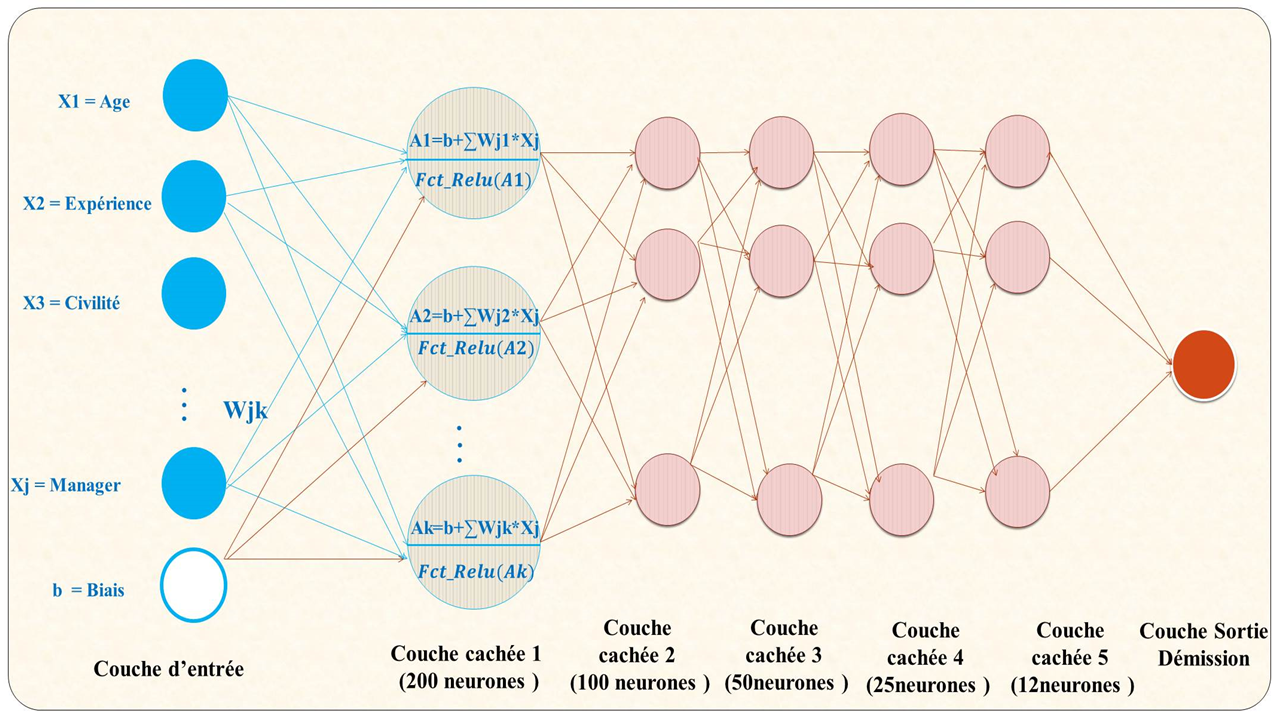
\includegraphics[width=1\linewidth]{img/DeepLearning.png}}
    \caption{Architecture de notre réseau de neurones}
    \label{fig:deeplearning}
    \end{figure}
    \\
Après plusieurs tentatives, nous avons fixé notre architecture de réseau de neurones qui répond à notre besoin (couche d’entrée + 5 couches cachées + couche de sortie).
Pour mieux comprendre cette architecture, notre réseau de neurones est composé de : 

\begin{itemize}
    \item une couche d'entrée : cette couche contient les variables explicatives concernant les informations des employés  ( civilité, expérience avant sofrecom, expérience sofrecom, expérience totale, séniorité, niveau académique, poste, pôle, manager, âge, situation familiale );
    \item b : biais;
    \item un système de poids (Wjk) liés à ces entrées;
    \item cinq couches cachées comportant respectivement 200,100,50,25,12 neurones;
     \item couche de sortie : démission (la variable cible ou expliquée);   
     \item fonction d'activation « Relu » dans chaque neurone de couche cachée : Relu est une fonction d'activation non linéaire la plus simple et la plus utilisée.
     \newpage
     Cette fonction d'activation transforme la sortie en 0 si l'entrée est inférieure à 0 sinon la sortie est égale à l'entrée comme le montre la figure \ref{fig:relu}.
        \begin{figure}[htpb]
    \centering
    \fcolorbox{brown}{white}{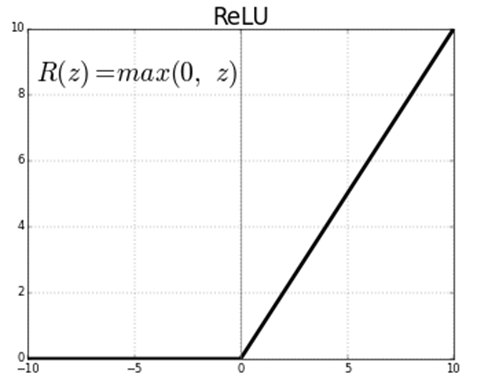
\includegraphics[width=0.75\linewidth]{img/relu2.png}}
    \caption{Fonction d'activation « Relu »}
    \label{fig:relu}
    \end{figure}


\end{itemize}
\subsubsection{Évaluation du modèle}
La phase d'évaluation du modèle est la plus importante pour avoir une bonne visualisation sur la performance de notre modèle.
En effet, lors de la création de notre modèle, Tensorflow nous donne des indications sur la valeur de la fonction d'erreur (loss) pendant chaque itération comme le montre la figure \ref{fig:eval}.
     \begin{figure}[htpb]
    \centering
    \fcolorbox{brown}{white}{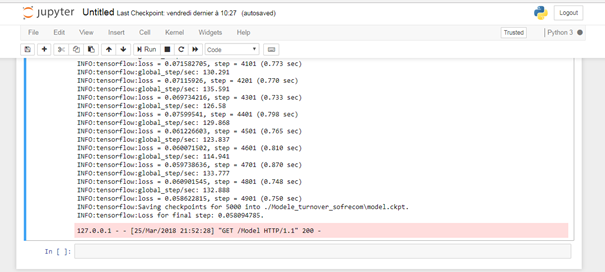
\includegraphics[width=0.75\linewidth]{img/env3.png}}
    \caption{Évaluation de notre modèle de réseau de neurones}
    \label{fig:eval}
    \end{figure}
    \\
Notre fonction d'erreur (loss) est définie par défaut dans Tensorflow comme étant l'erreur quadratique moyenne.\\
En effet, tensorflow offre un outil performant « Tensorboard » qui nous permet de visualiser les différentes valeurs de la fonction d’erreur pendant chaque itération comme le montre la figure \ref{fig:tensorboard}.
     \begin{figure}[htpb]
    \centering
    \fcolorbox{brown}{white}{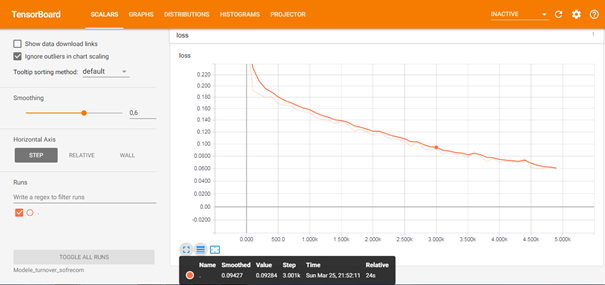
\includegraphics{img/tensorboard_.png}}
    \caption{Visualisation de la fonction d'erreur avec « Tensorboard »}
    \label{fig:tensorboard}
    \end{figure}
    \\
La fonction d’erreur est égale à 0.23 pendant la première itération et elle a diminué à 0.09284 dans l’itération 3000.\\La valeur de notre fonction d’erreur finale est égale à 0.05 dans l’itération 5000.\\
\textbf{Prédiction des données de test sur notre modèle}\\
Nous allons tester la performance de notre modèle avec les données de test.
Comme le montre la figure \ref{fig:predictiontest1}, les données réelles des employés ainsi que la valeur de leur démission.
     \begin{figure}[htpb]
    \centering
    \fcolorbox{brown}{white}{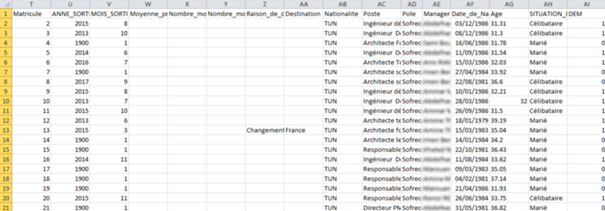
\includegraphics{img/pred1.png}}
    \caption{Visualisation des informations réelles des employés}
    \label{fig:predictiontest1}
    \end{figure}
    \newpage
Nous allons appliquer la prédiction sur notre modèle construit.
La figure \ref{fig:predictiontest2} nous montre la variable de démission prédite pour chaque employé.
     \begin{figure}[htpb]
    \centering
    \fcolorbox{brown}{white}{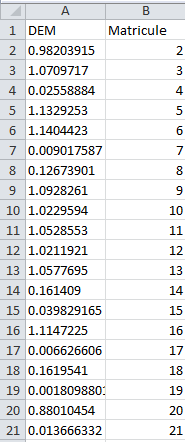
\includegraphics{img/pred2.png}}
    \caption{Visualisation des sorties prédites des employés}
    \label{fig:predictiontest2}
    \end{figure}
    \\
Ce modèle répond parfaitement à notre problème avec un taux de précision de 0.95.

\subsubsection{Réalisation}
Dans cette partie, nous allons exposer l'interface d'import du fichier contenant les informations des employés pour la construction de notre modèle et dont nous voulons effectuer des prédictions comme le montre la figure \ref{fig:importdata}.
\newpage
     \begin{figure}[htpb]
    \centering
    \fcolorbox{brown}{white}{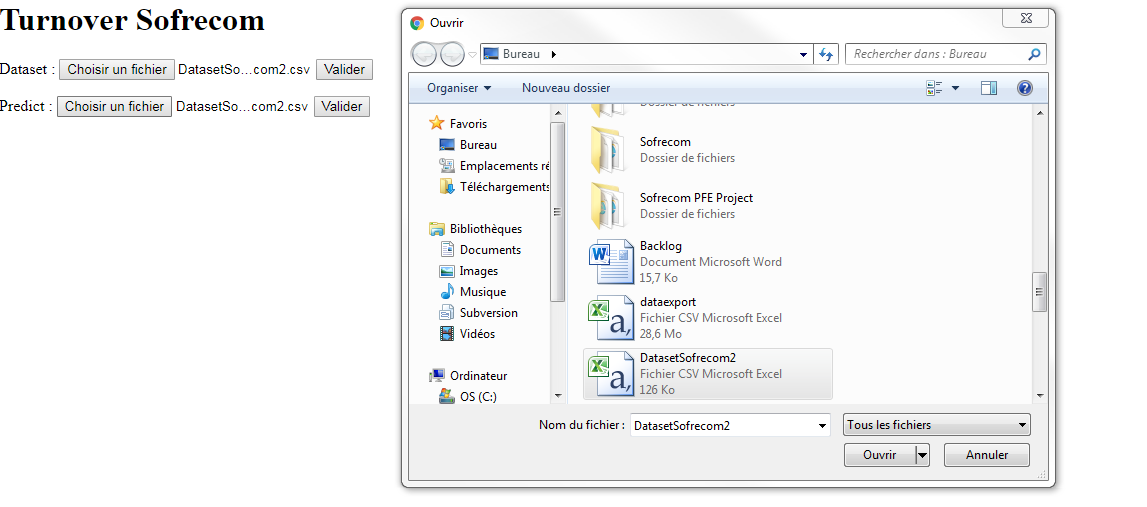
\includegraphics[width=1\linewidth]{img/import1.png}}
    \caption{Interface d'import des données}
    \label{fig:importdata}
    \end{figure}

Les différentes phases que nous avons abordées précédemment (préparation des données, division des données, création du modèle, prédiction) sont exposées sous format de service web.
Exemple d'appel du service web de division des données comme le montre la figure \ref{fig:splitdata2}.

     \begin{figure}[htpb]
    \centering
    \fcolorbox{brown}{white}{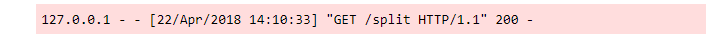
\includegraphics[width=1\linewidth]{img/pre4.png}}
    \caption{Appel de service web de division des données}
    \label{fig:splitdata2}
    \end{figure}

Exemple du résultat retourné du service web de prédiction comme le montre la figure \ref{fig:preddata}.
     \begin{figure}[htpb]
    \centering
    \fcolorbox{brown}{white}{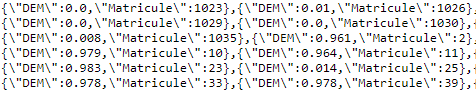
\includegraphics[width=1\linewidth]{img/pred3.png}}
    \caption{Résultat retourné de service web de prédiction}
    \label{fig:preddata}
    \end{figure}
    \newpage

\newpage
\section{Sprint 2 Gestion des prédictions des employés}
Ce sprint a pour but de développer les deux modules de notre application qui sont la gestion des prédictions et la gestion des employés.
\subsection{Backlog du Sprint}
Une fois, nous avons défini le but de notre sprint, il est temps de décider quelles sont les user story à inclure dans ce dernier.\\
Le tableau 4.6 résume le backlog de notre deuxième sprint :
\captionof{table}{Backlog du Sprint 2}

\begin{tabular}{@{}| >{\centering\arraybackslash}p{.04\textwidth}| >{\centering\arraybackslash}p{.30\textwidth}|>{\centering\arraybackslash}p{.06\textwidth}| >{\centering\arraybackslash}p{.35\textwidth}| >{\centering\arraybackslash}p{.13\textwidth}|@{}}

\hline \rowcolor{lightgray} \textbf{ID}  &  \textbf { User Story} & \textbf {ID Tâche} & \textbf {Tâche} & \textbf{Estimation (jours)} \\



\hline

\multirow{4}{*}{6} & \multirow{4}{.30\textwidth}{En tant qu’utilisateur, je veux
effectuer une prédiction sur la
démission d’un employé.}  & 6.1 
  & Création de l’interface de prédiction sur la démission des employés. & 1 \\ 
\cline{3-5}
& &  6.2 & Implémenter les méthodes nécessaires pour
l'appel de service web de prédiction et l'affichage de son résultat. & 1 \\
\cline{3-5}
& &  6.3 & Tester l'affichage de prédiction. & 1 \\


\hline



\multirow{4}{*}{7} & \multirow{4}{.30\textwidth}{En tant qu’utilisateur, je souhaite
consulter la liste des employés prédits.}  & 7.1 
  & Création de l’interface graphique de
consultation. & 1 \\ 
\cline{3-5}
& &  7.2 & Implémenter les méthodes nécessaires pour la
consultation. & 1 \\
\cline{3-5}
& &  7.3 & Tester la consultation de la liste des employés prédits. & 1 \\


\hline

\multirow{4}{*}{8} & \multirow{4}{.30\textwidth}{En tant qu’utilisateur, je souhaite
exporter l'historique des prédictions d'un employé sous format PDF.}  & 8.1 
  & Création de l’interface graphique de
consultation de l'historique des prédictions.& 1 \\ 
\cline{3-5}
& &  8.2 & Implémenter les méthodes nécessaires pour la
consultation. & 1 \\


\hline
\end{tabular}



%second table %
\begin{tabular}{@{}| >{\centering\arraybackslash}p{.04\textwidth}| >{\centering\arraybackslash}p{.30\textwidth}|>{\centering\arraybackslash}p{.06\textwidth}| >{\centering\arraybackslash}p{.35\textwidth}| >{\centering\arraybackslash}p{.13\textwidth}|@{}}

\hline \rowcolor{lightgray} \textbf{ID}  &  \textbf { User Story} & \textbf {ID Tâche} & \textbf {Tâche} & \textbf{Estimation (jours)} \\



\hline

{} & {}  & 8.3
  & Tester la consultation de l'historique des prédictions. & 1 \\ 


\hline



\multirow{4}{*}{9} & \multirow{4}{.32\textwidth}{En tant qu’utilisateur, je souhaite
rechercher la liste des employés prédits.}  & 9.1 
  &  Implémenter les méthodes nécessaires pour la
recherche. & 1 \\ 

\cline{3-5}
& &  9.2 & Tester la recherche des prédictions des employés. & 1 \\


\hline

\multirow{4}{*}{10} & \multirow{4}{.30\textwidth}{En tant qu’utilisateur, je veux
ajouter un employé.}  & 10.1 
  & Création de l’interface graphique d'ajout d'un employé.& 1 \\ 
\cline{3-5}
& &  10.2 & Implémenter les méthodes nécessaires pour l'ajout. & 1 \\

\cline{3-5}
& &  10.3 & Tester l’ajout d'un employé. & 1 \\
\hline

\multirow{4}{*}{11} & \multirow{4}{.30\textwidth}{En tant qu’utilisateur, je veux
modifier un employé.}  & 11.1 
  & Création de l’interface graphique de
modification d'un employé.& 1 \\ 
\cline{3-5}
& &  11.2 & Implémenter les méthodes nécessaires pour la modification. & 1 \\

\cline{3-5}
& &  11.3 & Tester la modification d'un employé. & 1 \\
\hline



\multirow{4}{*}{12} & \multirow{4}{.30\textwidth}{En tant qu’utilisateur, je veux
supprimer un employé.}  & 12.1 
  & Création d'un message d'alerte pour la confirmation de suppression d'un employé.& 1 \\ 
\cline{3-5}
& &  12.2 & Implémenter les méthodes nécessaires pour la suppression. & 1 \\

\cline{3-5}
& &  12.3 & Tester la suppression d'un employé. & 1 \\

\hline


\multirow{4}{*}{13} & \multirow{4}{.32\textwidth}{En tant qu’utilisateur, je souhaite
consulter et effectuer une recherche
sur la liste des employés.}  & 13.1 
  &  Implémenter les méthodes nécessaires pour la
recherche d'un employé. & 1 \\ 

\cline{3-5}
& &  13.2 & Tester la recherche des employés. & 1 \\

\hline
\end{tabular}





%third table %
\begin{tabular}{@{}| >{\centering\arraybackslash}p{.04\textwidth}| >{\centering\arraybackslash}p{.30\textwidth}|>{\centering\arraybackslash}p{.06\textwidth}| >{\centering\arraybackslash}p{.35\textwidth}| >{\centering\arraybackslash}p{.13\textwidth}|@{}}

\hline \rowcolor{lightgray} \textbf{ID}  &  \textbf { User Story} & \textbf {ID Tâche} & \textbf {Tâche} & \textbf{Estimation (jours)} \\



\hline




\multirow{4}{*}{14} & \multirow{4}{.31\textwidth}{En tant qu’utilisateur, je souhaite
exporter  toutes  les  informations
d’un employé sous format PDF.}  & 14.1 
  &  Implémenter les méthodes nécessaires pour l'exportation des informations d'un employé. & 1 \\ 

\cline{3-5}
& &  14.2 & Tester le format d'exportation. & 1 \\


\hline


\end{tabular}






\subsection{Spécification fonctionnelle}
La figure \ref{fig:useCaseSprint2_1} présente le diagramme de cas d’utilisation détaillé de «Gérer les prédictions».
 \begin{figure}[htpb]
    \centering
    \fcolorbox{brown}{white}{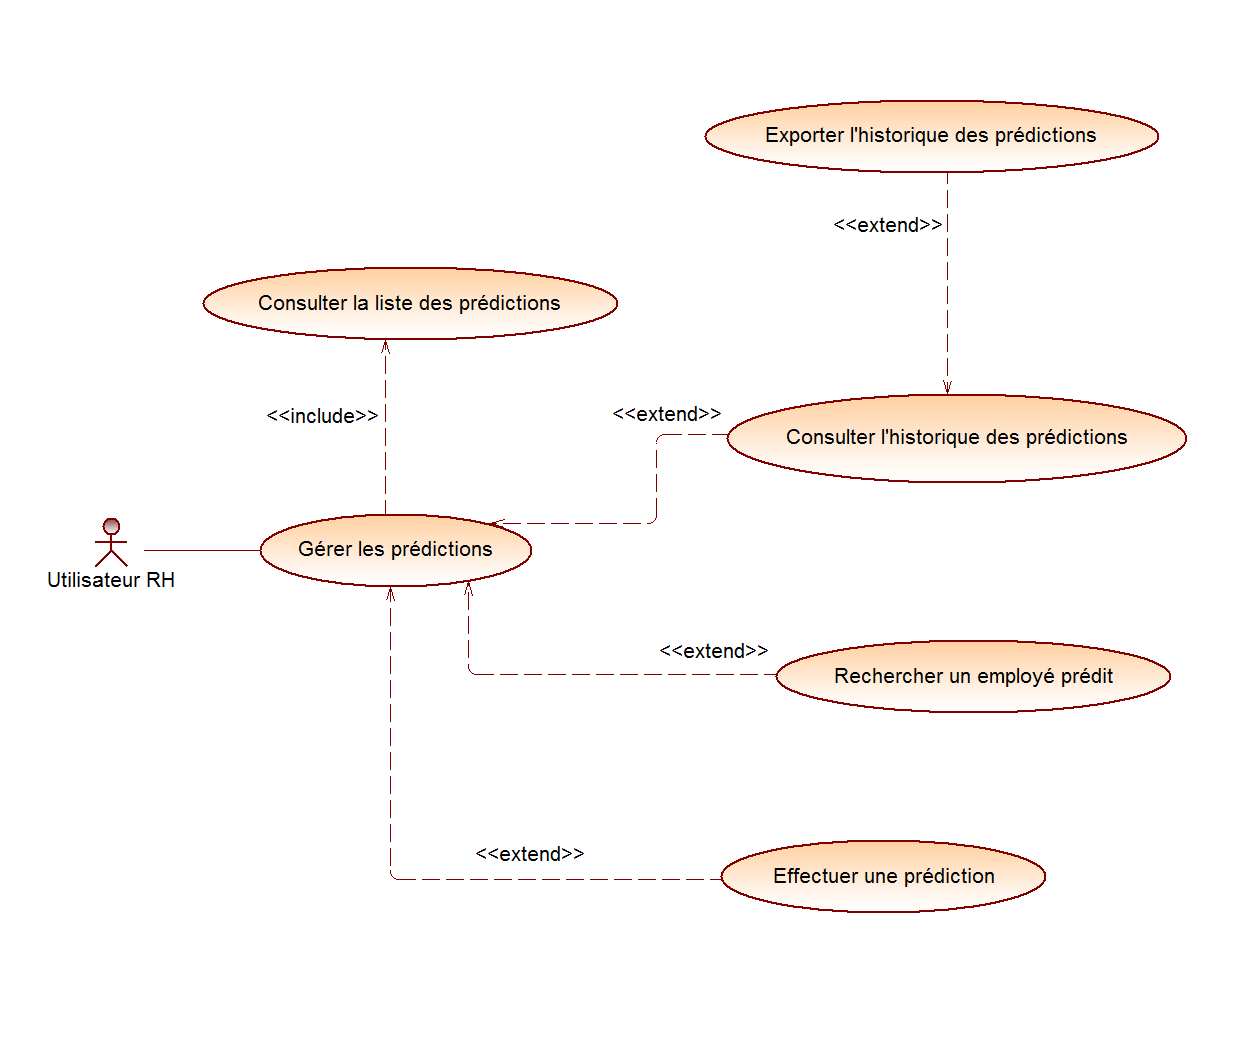
\includegraphics[width=1\linewidth]{img/release1sprint2_1_final.png}}
    \caption{Diagramme de cas d’utilisation « Gérer les prédictions »}
    \label{fig:useCaseSprint2_1}
    \end{figure}
    
\newpage
La figure \ref{fig:useCaseSprint2_2} présente le diagramme de cas d’utilisation détaillé de «Gérer les employés».
\begin{figure}[htpb]
    \centering
    \fcolorbox{brown}{white}{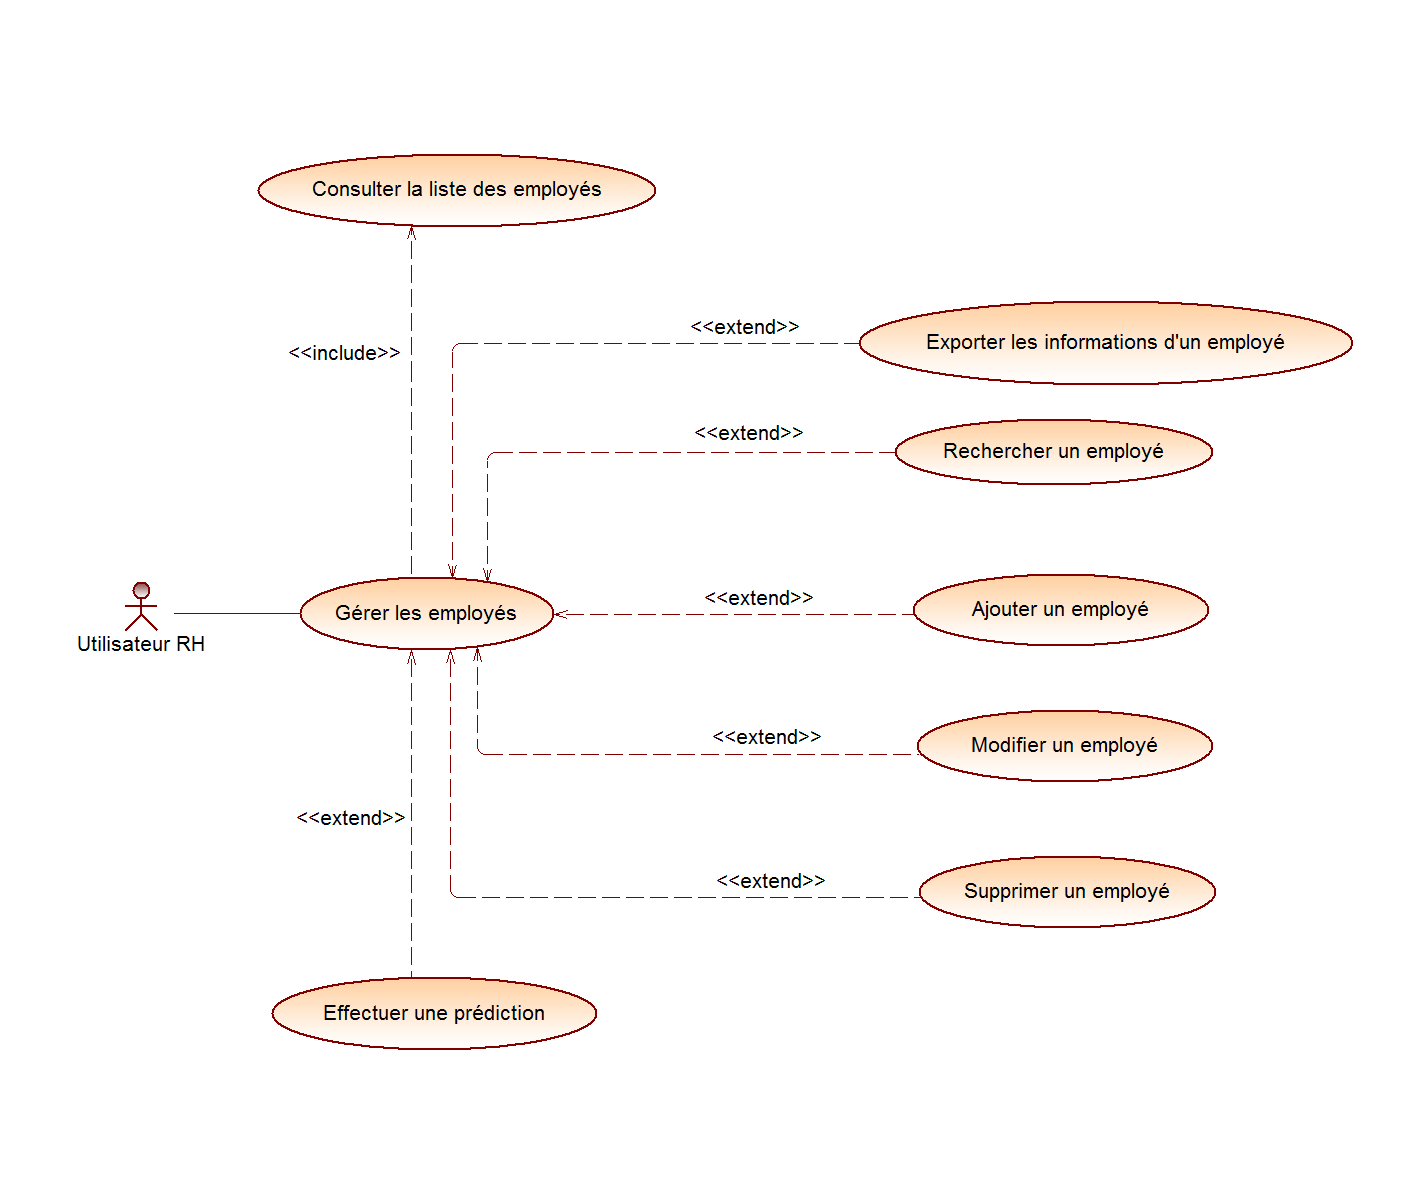
\includegraphics[width=1\linewidth]{img/release1sprint2_2_final.png}}
    \caption{Diagramme de cas d’utilisation « Gérer les employés »}
    \label{fig:useCaseSprint2_2}
    \end{figure}
\newline Le tableau \ref{tab:Effectueruneprediction} présente la description textuelle du cas d’utilisation « Effectuer une prédiction ».
\begin{longtable}[c]{
    |p{.25\textwidth}
    |p{.71\textwidth}|
}
    \caption{Description du diagramme de cas d’utilisation <<Effectuer une prédiction>>}
    \label{tab:Effectueruneprediction}\\
    \hline
    
    Cas d’utilisation
    & Effectuer une prédiction. \\
    \hline 
    
    Acteur
    & Utilisateur RH ou l'administrateur. \\
    \hline 
    
    Précondition
    & L'utilisateur doit accéder à l'interface de gestion des prédictions ou gestion des employés. \\
    \hline
    
    Post-condition
    & Prédiction effectuée avec succès. \\
    \hline
    
    Description du
scénario

    &     \begin{itemize}
    \item L’utilisateur choisit un employé.
    \item Le système renvoie un message d'alerte pour confirmer la prédiction.
     \item L'utilisateur confirme la prédiction de l'employé choisi.
     \item Le système enregistre le résultat de la prédiction et affiche un message de succès de l'opération.

    \end{itemize} \\
    \hline
    
   Exception
    & Erreur de connexion.
 \\ \hline
   
\end{longtable}





%second table description%
Le tableau \ref{tab:exportinfoemployé} présente la description textuelle du cas d’utilisation « Exporter les informations d'un employé ».
\begin{longtable}[c]{
    |p{.25\textwidth}
    |p{.71\textwidth}|
}
    \caption{Description du diagramme de cas d’utilisation <<Exporter les informations d'un employé>>}
    \label{tab:exportinfoemployé}\\
    \hline
    
    Cas d’utilisation
    &  Exporter les informations d'un employé. \\
    \hline 
    
    Acteur
    & Utilisateur RH ou l'administrateur. \\
    \hline 
    
    Précondition
    & L'utilisateur doit accéder à l'interface de gestion des employés. \\
    \hline
    
    Post-condition
    & Fichier PDF téléchargé. \\
    \hline
    
    Description du
scénario

    &     \begin{itemize}
    \item L’utilisateur choisit un employé à exporter ses informations.
    \item Le système affiche un message de confirmation.
     \item L'utilisateur confirme l'exportation des informations de l'employé choisi.
     \item Le système retourne un fichier PDF contenant toutes les informations de l'employé choisi.

    \end{itemize} \\
    \hline
    
   Exception
    & Erreur de connexion.
 \\ \hline
   
\end{longtable}

\newpage

% Third Description %
Le tableau \ref{tab:Ajouteremployé} présente la description textuelle du cas d’utilisation « Ajouter un employé ».
\begin{longtable}[c]{
    |p{.25\textwidth}
    |p{.71\textwidth}|
}
    \caption{Description du diagramme de cas d’utilisation <<Ajouter un employé>>}
    \label{tab:Ajouteremployé}\\
    \hline
    
    Cas d’utilisation
    &  Ajouter un employé. \\
    \hline 
    
    Acteur
    & Utilisateur RH ou l'administrateur. \\
    \hline 
    
    Précondition
    & L'utilisateur doit accéder à l'interface de gestion des employés. \\
    \hline
    
    Post-condition
    & Employé ajouté. \\
    \hline
    
    Description du
scénario

    &     \begin{itemize}
    \item L’utilisateur choisit d'ajouter un nouvel employé.
    \item Le système renvoie le formulaire d’ajout d’un nouvel employé.
       \item L’utilisateur remplit les champs nécessaires et valide la saisie.
     \item Le système enregistre les données et affiche un message
de succès.

    \end{itemize} \\
    \hline
    
   Exception
    & Erreur de connexion.
 \\ \hline
   
\end{longtable}




% 4th Description %
Le tableau \ref{tab:Supprimeremployé} présente la description textuelle du cas d’utilisation « Supprimer un employé ».
\begin{longtable}[c]{
    |p{.25\textwidth}
    |p{.71\textwidth}|
}
    \caption{Description du diagramme de cas d’utilisation <<Supprimer un employé>>}
    \label{tab:Supprimeremployé}\\
    \hline
    
    Cas d’utilisation
    &  Supprimer un employé. \\
    \hline 
    
    Acteur
    & Utilisateur RH ou l'administrateur. \\
    \hline 
    
    Précondition
    & L'utilisateur doit accéder à l'interface de gestion des employés. \\
    \hline
    
    Post-condition
    & Employé et ses prédictions sont supprimés . \\
    \hline
    
    Description du
scénario

    &     \begin{itemize}
    \item L’utilisateur choisit de supprimer un employé.
    \item Le système affiche un message de confirmation de suppression.

   \item L'utilisateur confirme la suppression de l'employé choisi.
     \item Le système supprime l'employé et ses prédictions et affiche un message de succès.
    \end{itemize} \\
    \hline
    
   Exception
    & Erreur de connexion.
 \\ \hline
   
\end{longtable}
\newpage
\textbf{Diagramme de séquences système de l’opération «Effectuer une prédiction»}\\
La figure \ref{fig:seqsystemepredictionEmploye} représente le diagramme de séquences système de l’opération «Effectuer une prédiction».
\begin{figure}[htpb]
    \centering
    \fcolorbox{brown}{white}{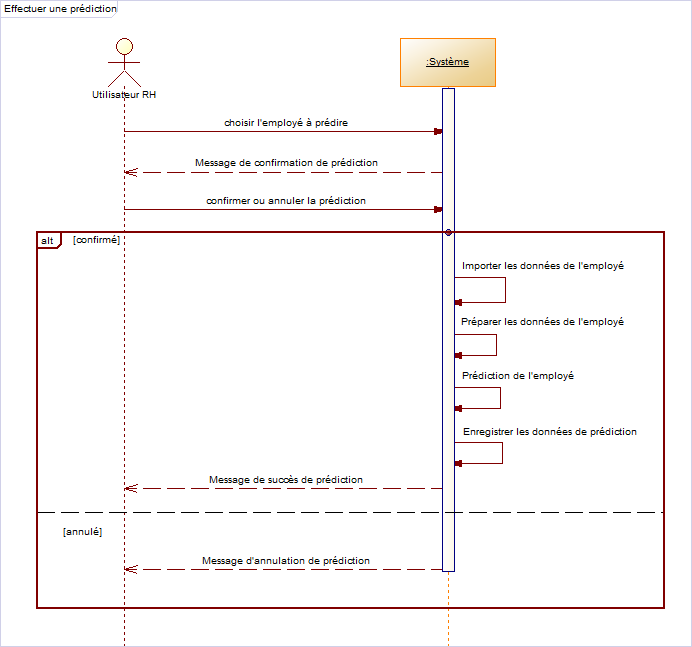
\includegraphics[width=16cm,height=40cm,keepaspectratio]{img/diagseqsystemepredictionEmploye.png}}
    \caption{Diagramme de séquences système « Effectuer une prédiction »}
    \label{fig:seqsystemepredictionEmploye}
    \end{figure}
\newpage
\textbf{Diagramme de séquences système de l’opération «Modifier un employé»}\\
La figure \ref{fig:seqsystemeModifierEmploye} représente le diagramme de séquences système de l’opération «Modifier un employé».
\begin{figure}[htpb]
    \centering
    \fcolorbox{brown}{white}{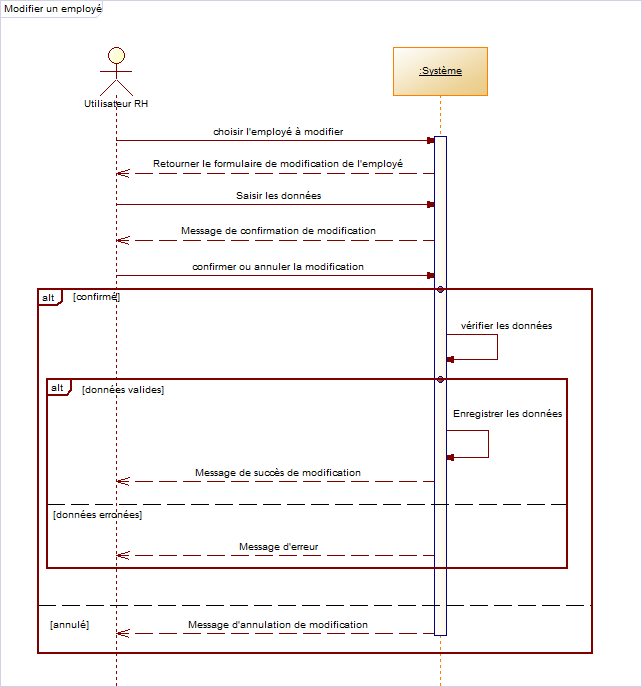
\includegraphics[width=16cm,height=40cm,keepaspectratio]{img/diagseqsystemeModifierEmploye.png}}
    \caption{Diagramme de séquences système « Modifier un employé »}
    \label{fig:seqsystemeModifierEmploye}
    \end{figure}
\newpage
\textbf{Diagramme de séquences système de l’opération «Supprimer un employé»}\\
La figure \ref{fig:seqsystemeSupprimerEmploye} représente le diagramme de séquences système de l’opération «Supprimer un employé».
\begin{figure}[htpb]
    \centering
    \fcolorbox{brown}{white}{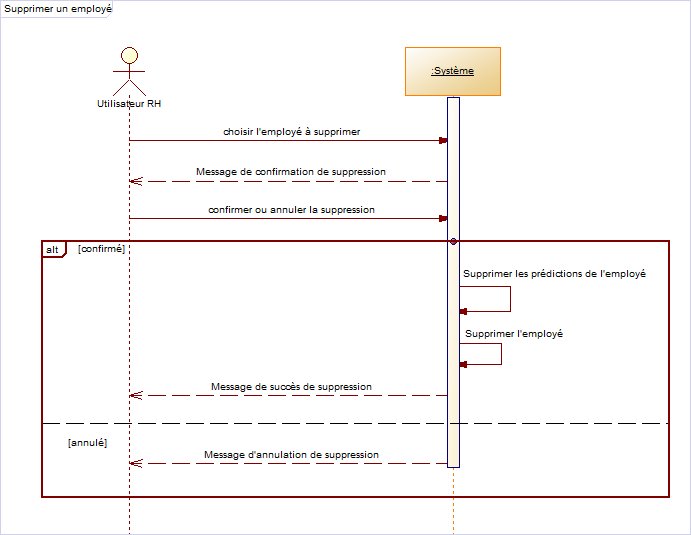
\includegraphics[width=16cm,height=40cm,keepaspectratio]{img/diagseqsystemesupprimerEmploye.png}}
    \caption{Diagramme de séquences système « Supprimer un employé »}
    \label{fig:seqsystemeSupprimerEmploye}
    \end{figure}
    

\subsection{Conception}
Dans cette section, nous allons présenter le diagramme de classe ainsi que les différents diagrammes de séquences détaillés.
   \subsubsection{Diagramme de classes}
  La figure \ref{fig:diagclasse3} définit les classes utilisées, pour mettre en place la gestion des prédictions et la gestion des employés.
\newpage

\begin{figure}[htpb]
    \centering
    \fcolorbox{brown}{white}{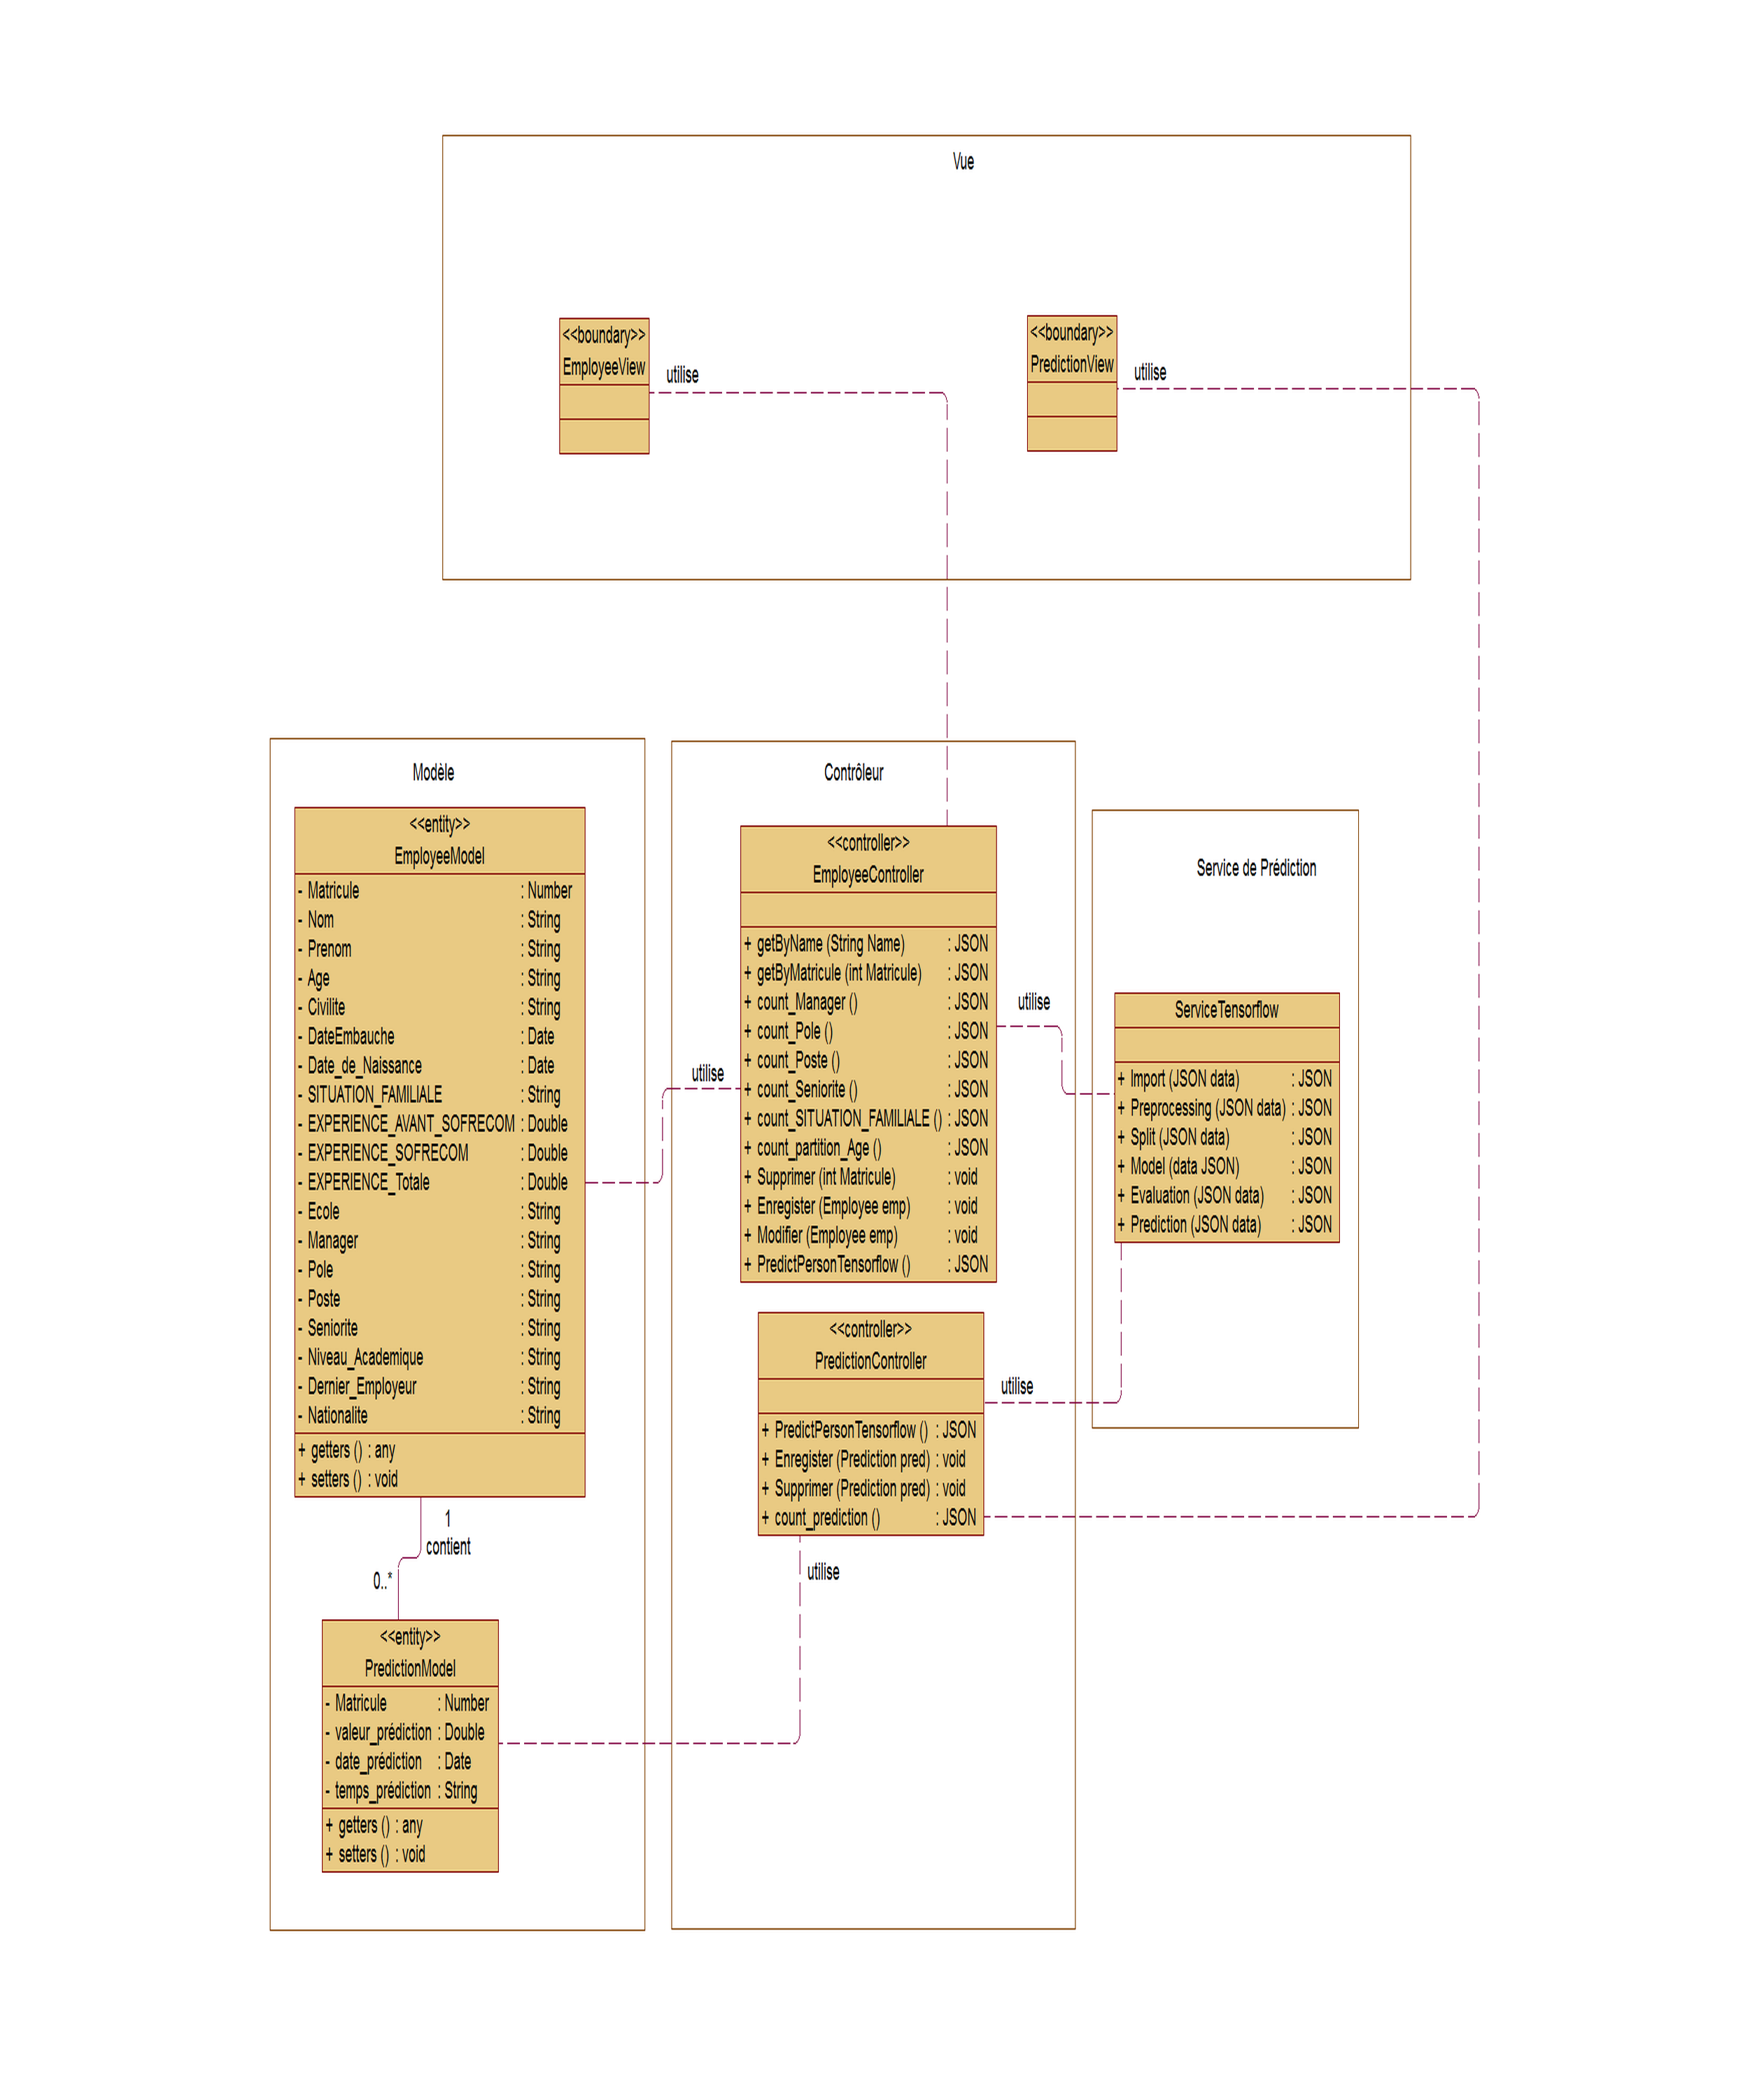
\includegraphics[width=1\linewidth]{img/diagclasse5.png}}
    \caption{Diagramme de classes}
    \label{fig:diagclasse3}
    \end{figure}

Pour mieux comprendre ce diagramme, les contrôleurs « EmployeeController » et \newline « PredictionController » jouent le rôle d'intermédiaire entre les entités, le service de prédiction et la vue qui interagit avec l'utilisateur.\newline
Au niveau du modèle, l'entité « EmployeeModel » peut contenir plusieurs prédictions et l'entité\newline « PredictionModel » est associée à un seul employé.\newline
La prédiction des démissions des employés est assurée par le service « ServiceTensorflow ».
\newpage
    \subsubsection{Diagrammes de séquences}
    Nous présentons dans ce qui suit les diagrammes de séquences détaillés du
deuxième sprint.\\
\textbf{Diagramme de séquences objet « Effectuer une prédiction »}\\
La prédiction est la fonctionnalité la plus importante dans notre application.\newline Pour effectuer ce traitement, l'utilisateur RH choisit un employé à prédire à partir de la vue\newline « PredictionView ». Le contrôleur « PredictionController » récupère les données de l'employé et invoque le service « ServiceTensorflow » pour effectuer la prédiction.\newline Une fois le traitement est terminé,
le contrôleur ordonne d'ajouter le résultat de l'opération dans l'entité  « PredictionModel » et le retourne à la vue.\newline
Un message de réussite sera affiché à l'utilisateur en indiquant le résultat de la prédiction.\newline
La figure \ref{fig:seqobjetprediction} décrit le déroulement du processus de la réalisation de cette tâche.
    \begin{figure}[htpb]
    \centering
    \fcolorbox{brown}{white}{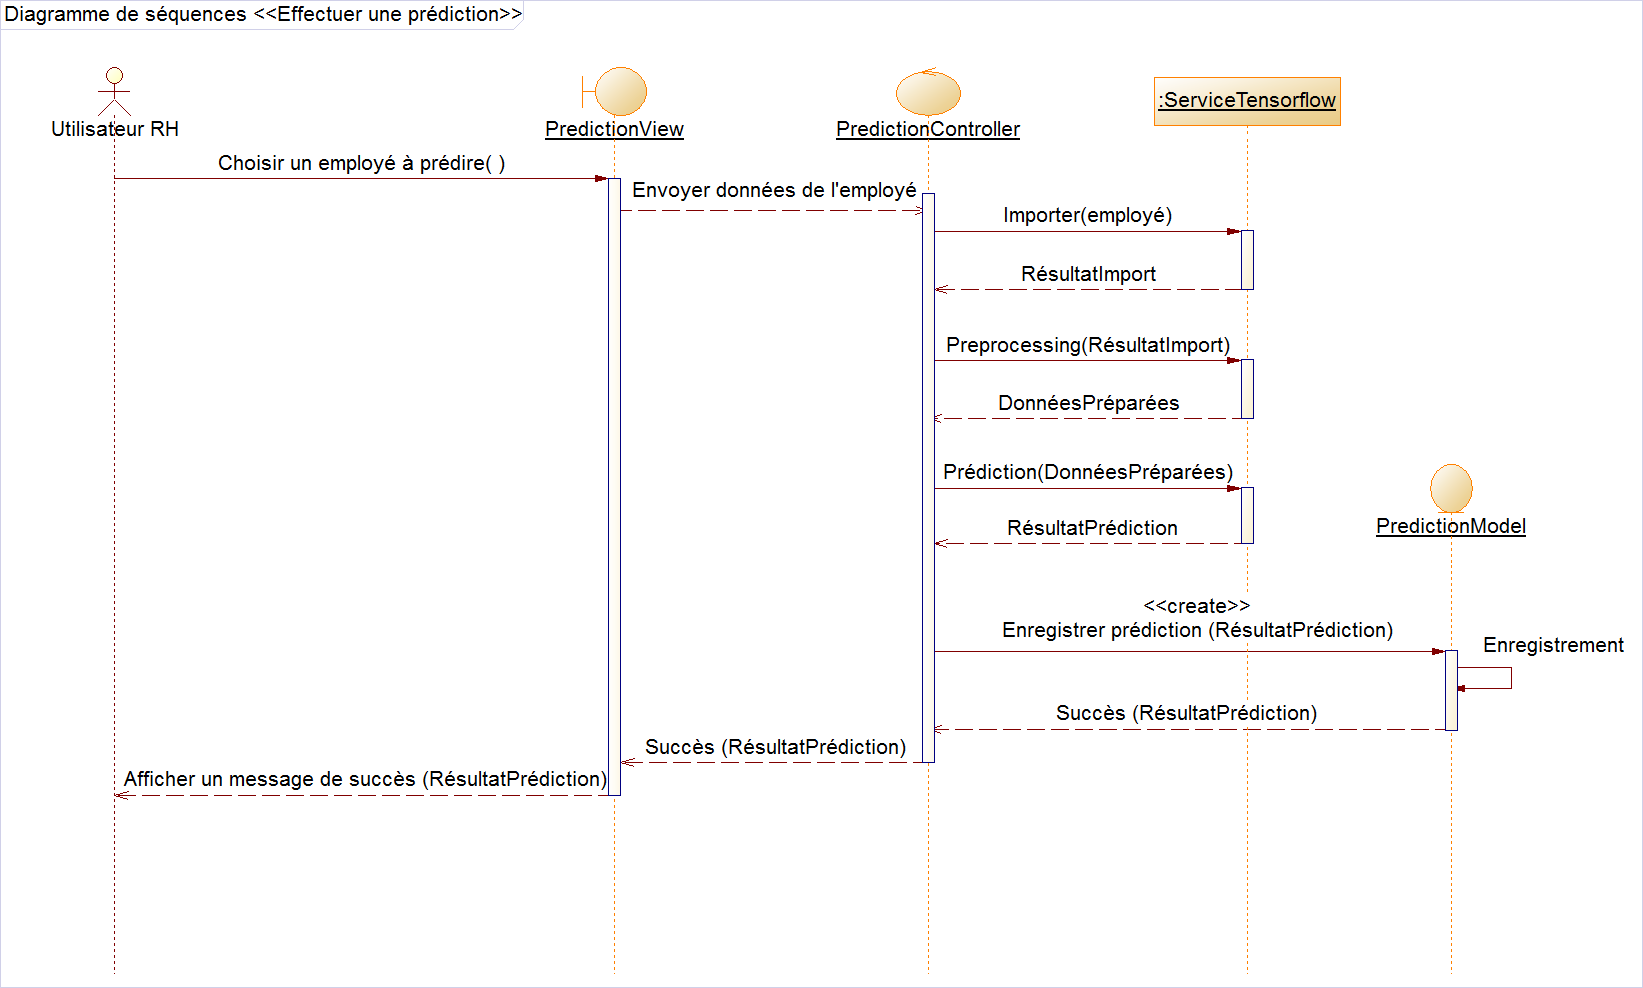
\includegraphics[width=1\linewidth]{img/seqobjetprediction_final.png}}
    \caption{Diagramme de séquences objet « Effectuer une prédiction »}
    \label{fig:seqobjetprediction}
    \end{figure}
    
    \newpage
\textbf{Diagramme de séquences objet « Modifier un employé »}\\
L’utilisateur RH peut modifier des données relatives à un employé déjà pris en charge par l’application. Il sélectionne l'employé à modifier à partir de l’interface « EmployeeView » et prend en charge les modifications à apporter.\newline Le contrôleur « EmployeeController » récupère les informations de l'employé et ordonne la mise à jour de l'employé dans l'entité « EmployeeModel ».\newline
La figure \ref{fig:seqobjetmodifemploye} expose le déroulement du processus de la réalisation de cette tâche.

    \begin{figure}[htpb]
    \centering
    \fcolorbox{brown}{white}{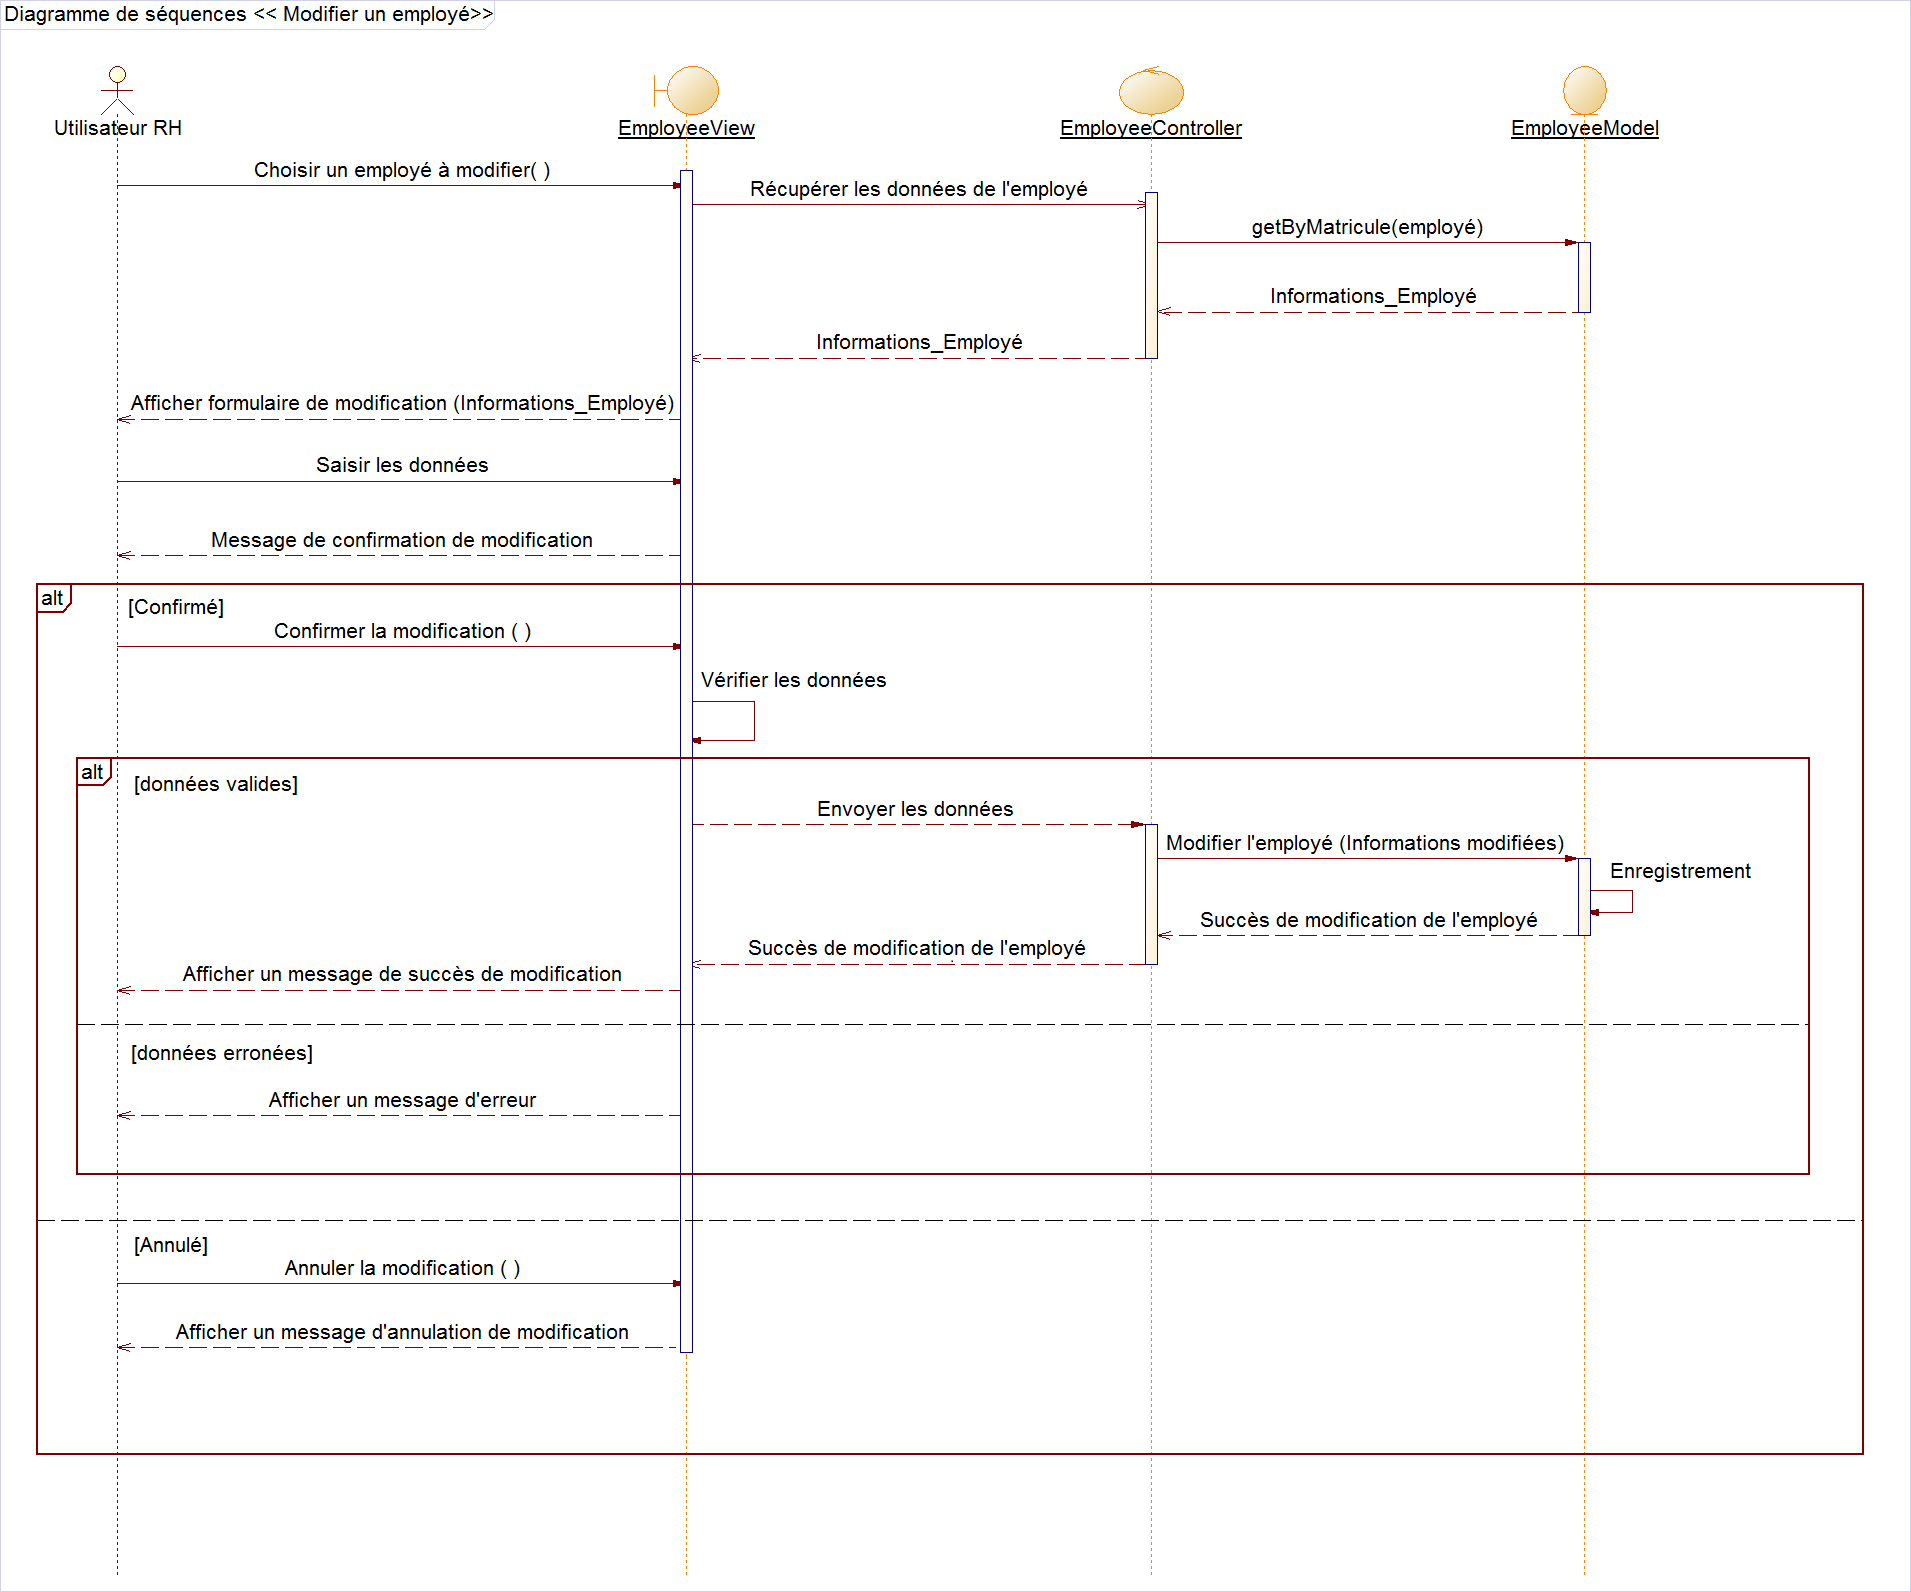
\includegraphics[width=1\linewidth]{img/seqobjetmodifemploye_final.png}}
    \caption{Diagramme de séquences objet « Modifier un employé »}
    \label{fig:seqobjetmodifemploye}
    \end{figure}
    
       \newpage

\textbf{Diagramme de séquences objet « Supprimer un employé »}\\
La suppression d’un employé est à la charge de l’utilisateur de l’application. Ce dernier sélectionne l'employé concerné à partir de l’interface « EmployeeView ». Une fois l'employé a été choisi, le contrôleur « EmployeeController » ordonne la suppression des prédictions associées à cet employé afin de respecter les contraintes d’intégrités et puis il ordonne la suppression de l'employé.\newline
La figure \ref{fig:seqobjetsupprimeremploye} illustre le déroulement du processus de la réalisation de cette tâche.
    \begin{figure}[htpb]
    \centering
    \fcolorbox{brown}{white}{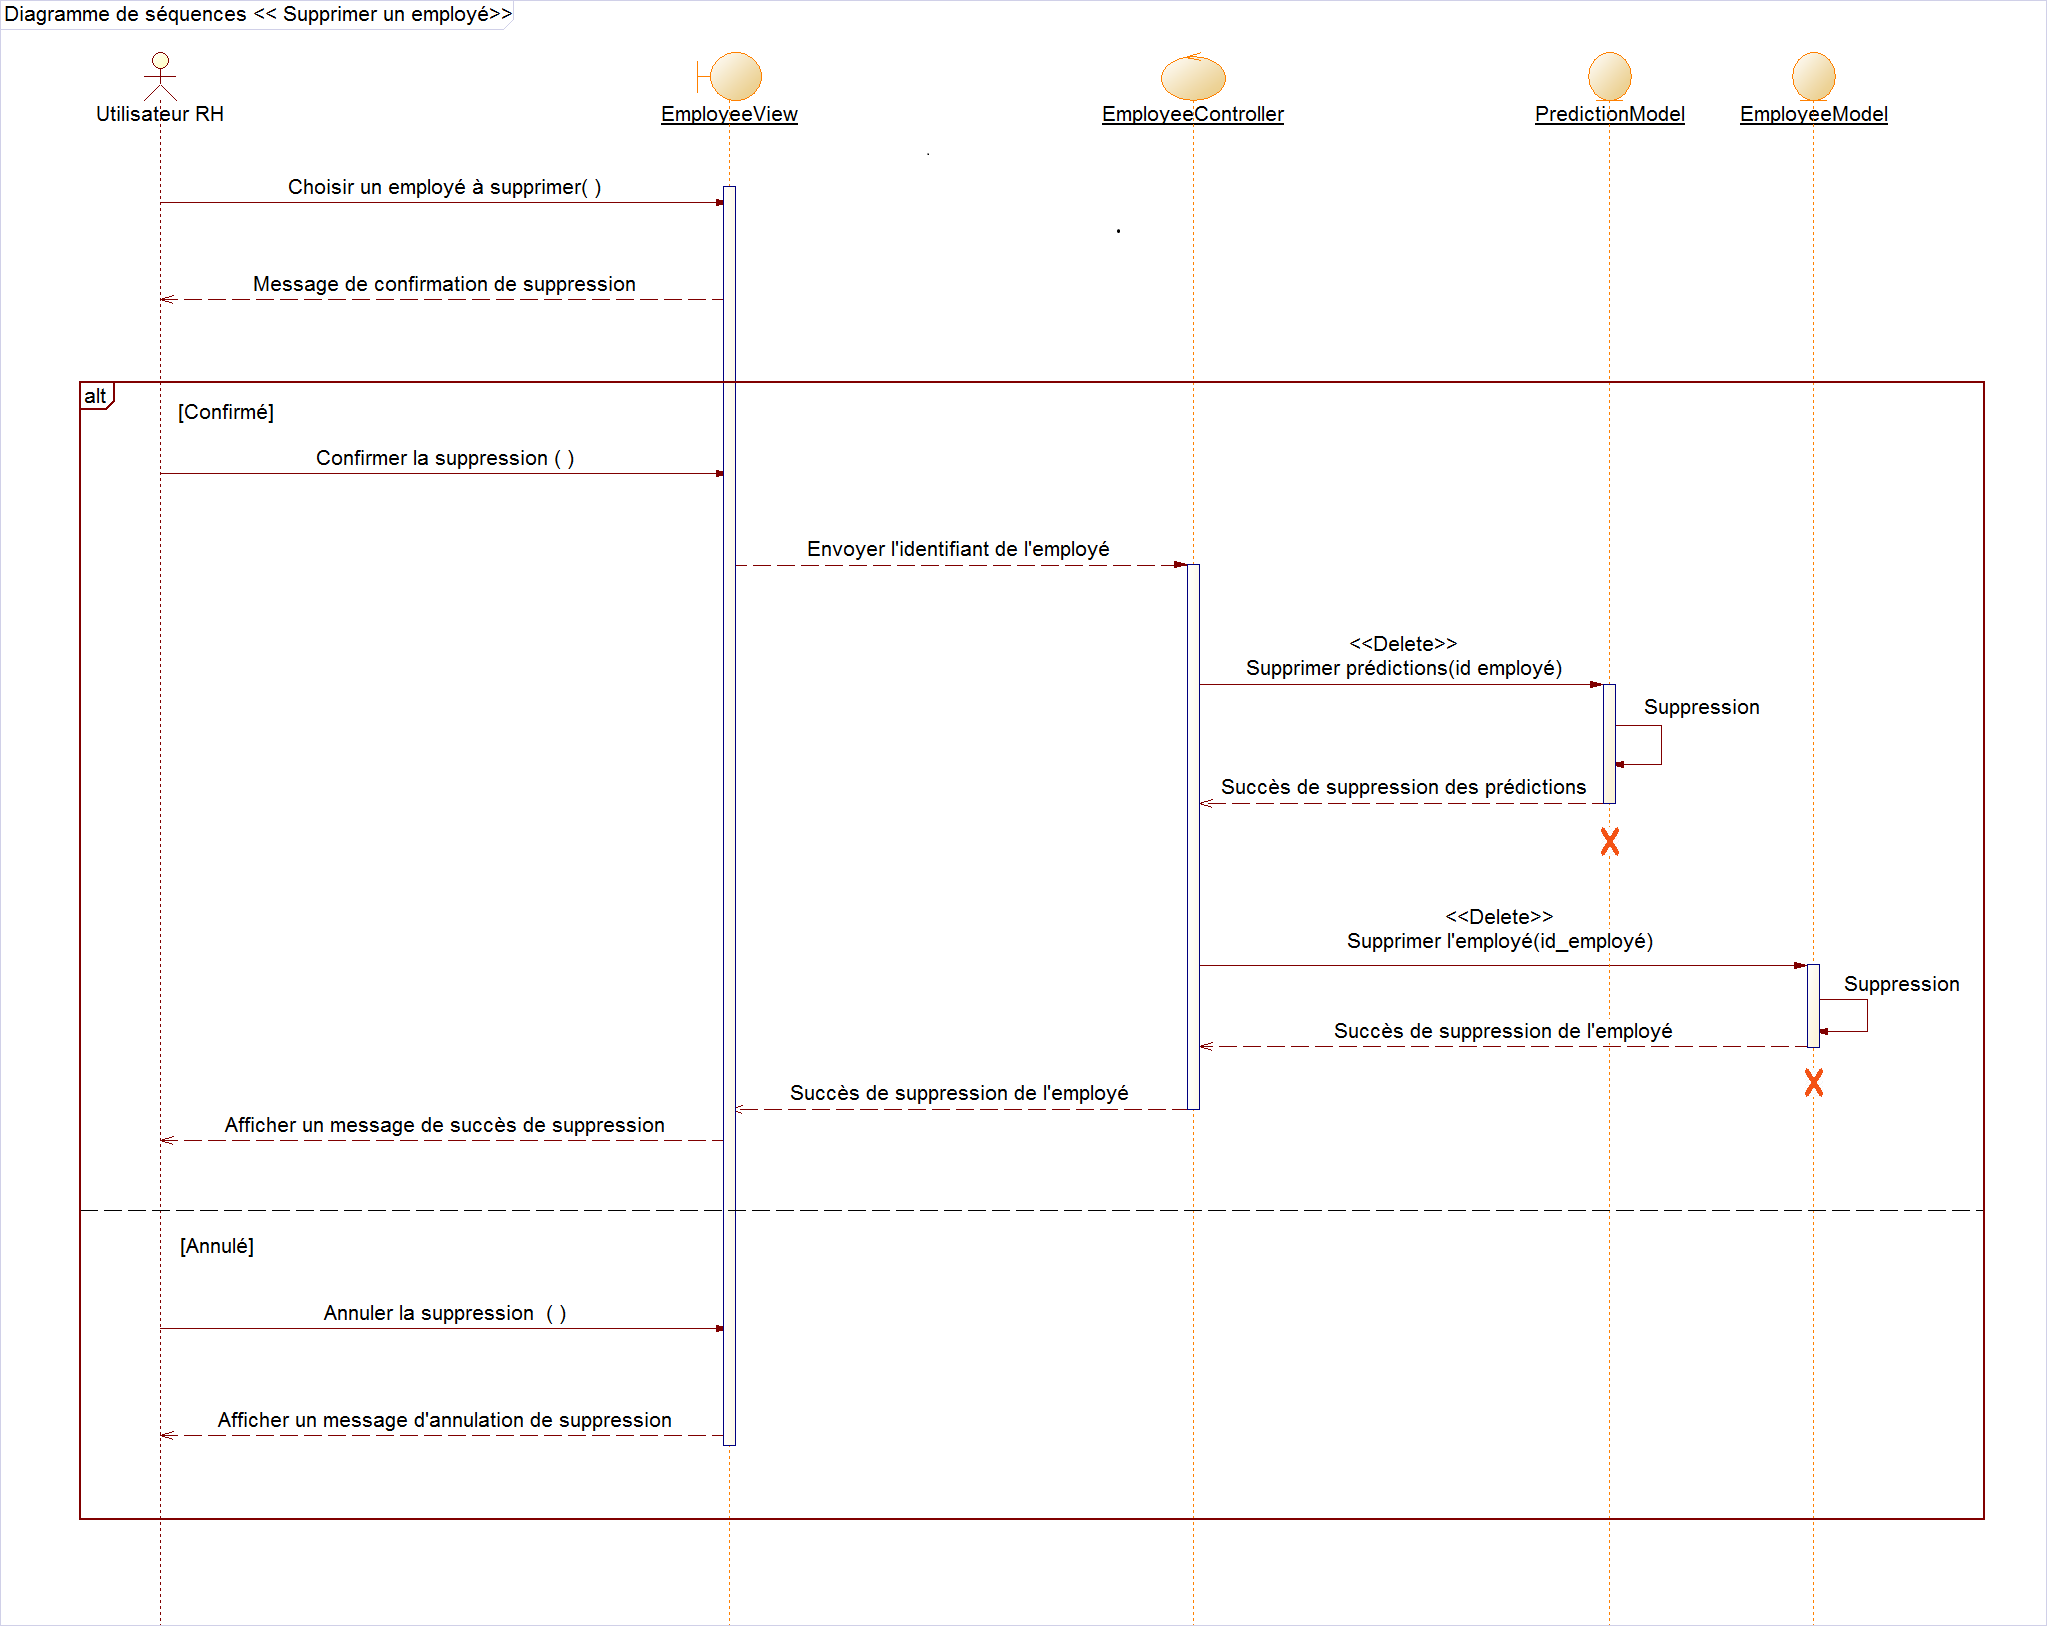
\includegraphics[width=1\linewidth]{img/SeqObjetSupprimerEmploye_final.png}}
    \caption{Diagramme de séquences objet « Supprimer un employé »}
    \label{fig:seqobjetsupprimeremploye}
    \end{figure}
    

\subsection{Réalisation}
Dans cette partie, nous allons exposer les différentes interfaces de notre application réalisées dans le deuxième
sprint.\newline
\textbf{Interface de gestion des employés}\\
L'utilisateur RH accède à la page de gestion des employés. Il peut consulter, ajouter, prédire, modifier, supprimer un employé ou exporter ses informations comme illustré sur la figure \ref{fig:realisationPFe_sprint2_0}.
\newpage

    \begin{figure}[htpb]
    \centering
    \fcolorbox{brown}{white}{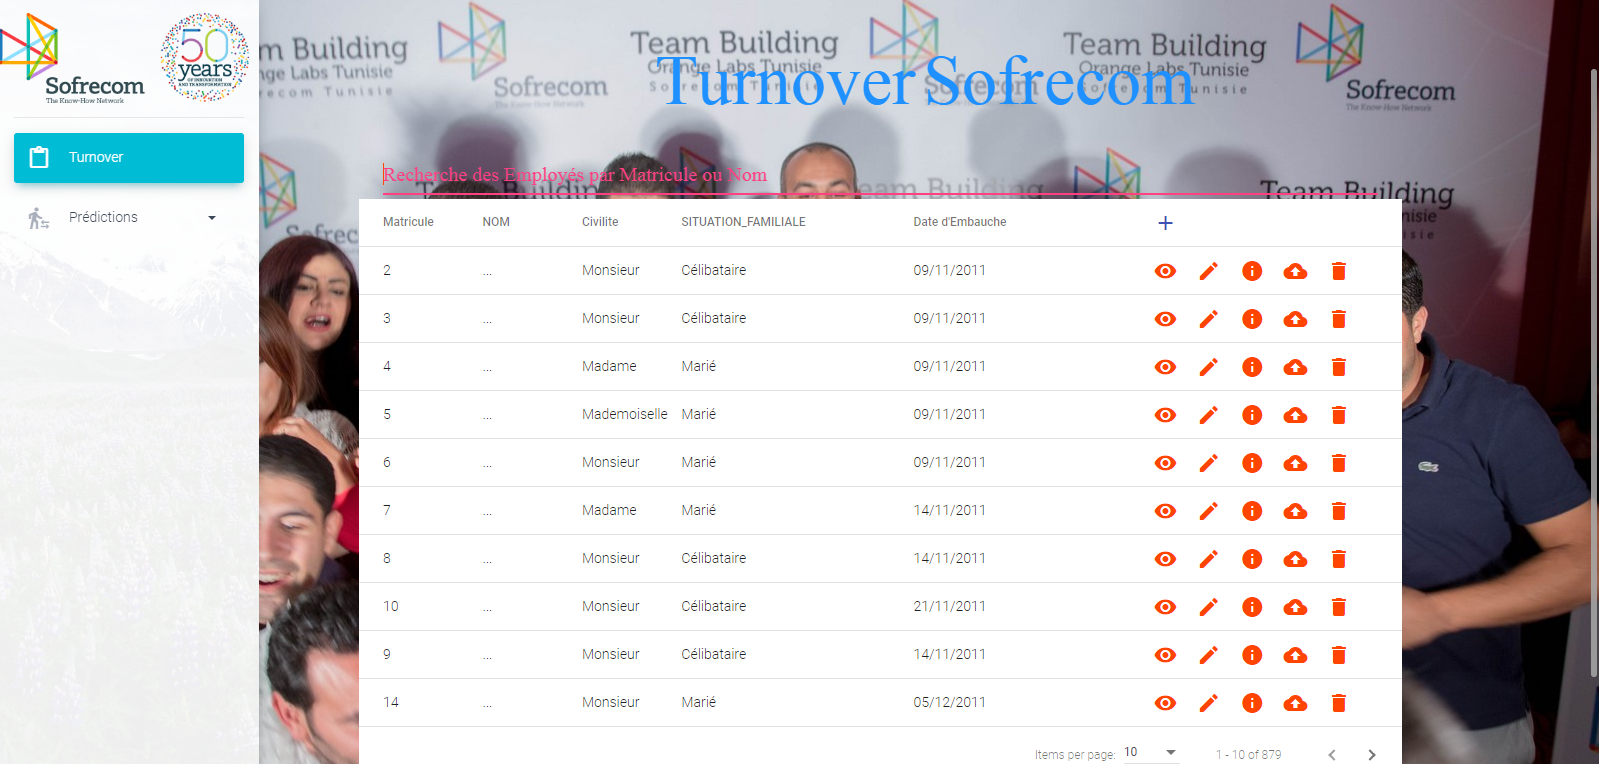
\includegraphics[width=1\linewidth]{img/realisationPFe_sprint2_0.png}}
    \caption{Interface de gestion des employés}
    \label{fig:realisationPFe_sprint2_0}
    \end{figure}

\textbf{Interface d'ajout d'un nouvel employé}\\
La figure \ref{fig:realisationPFe_sprint2_2} représente l'interface permettant à l'utilisateur RH d'ajouter un nouvel employé.\newline Le formulaire d'ajout contient plusieurs informations (nom, civilité, poste, manager...).
    \begin{figure}[htpb]
    \centering
    \fcolorbox{brown}{white}{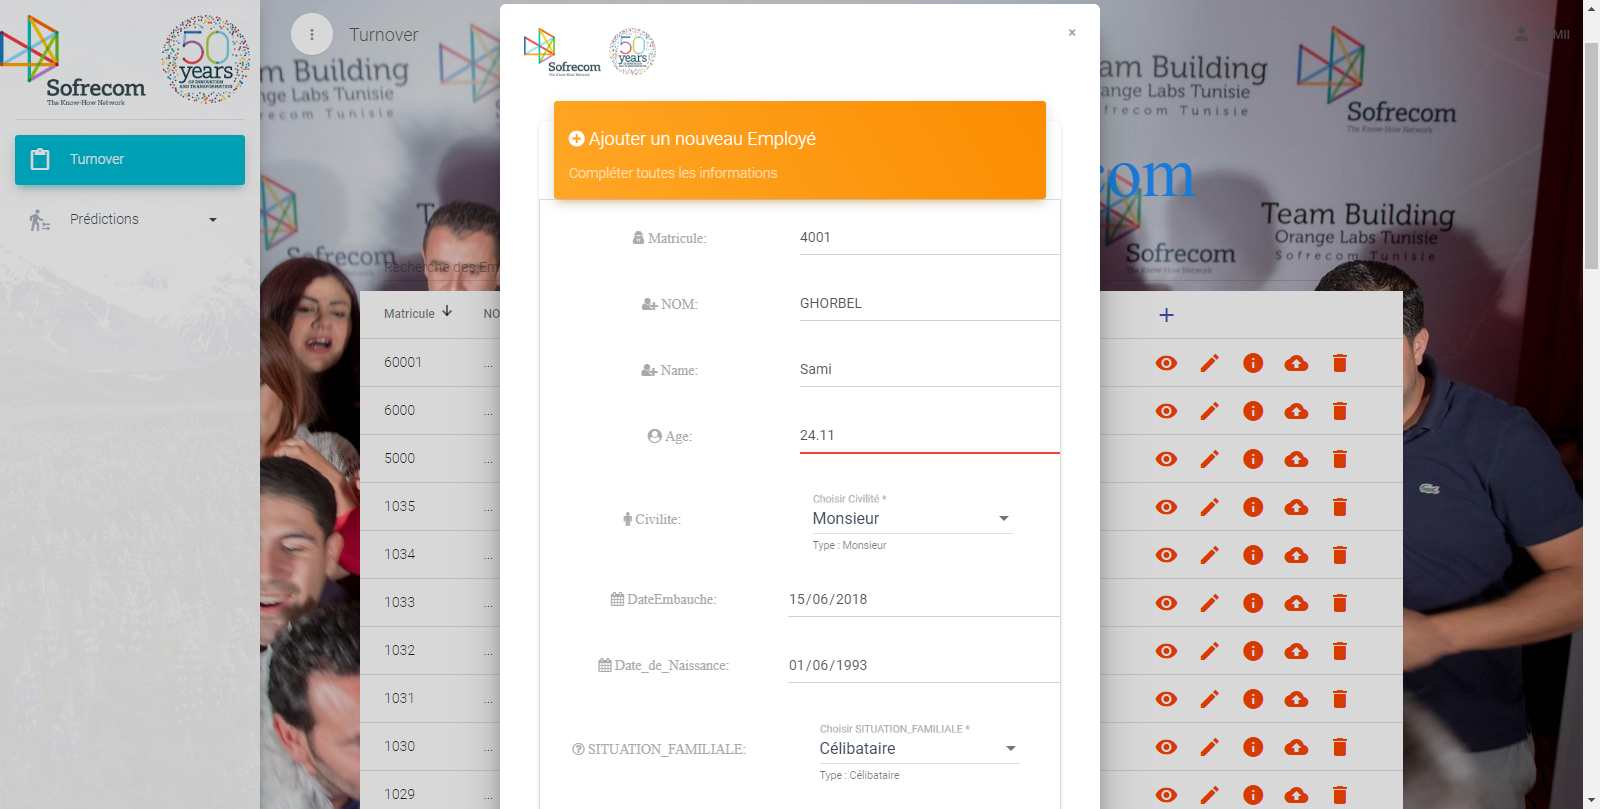
\includegraphics[width=1\linewidth]{img/realisationPFe_sprint2_2.png}}
    \caption{Interface d'ajout d'un nouvel employé}
    \label{fig:realisationPFe_sprint2_2}
    \end{figure}
 
 
\newpage   
\textbf{Interface de recherche d'un employé}\\
L'utilisateur RH peut effectuer une recherche d'un employé selon la matricule ou le nom de ce dernier comme illustré sur la figure \ref{fig:realisationPFe_sprint2_recherche}.

    \begin{figure}[htpb]
    \centering
    \fcolorbox{brown}{white}{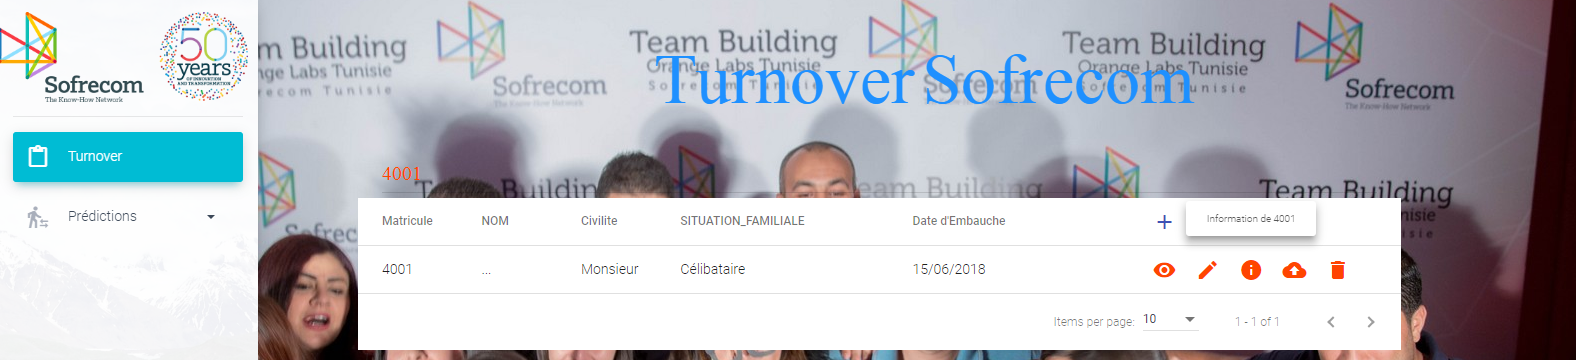
\includegraphics[width=1\linewidth]{img/realisationPFe_sprint2_recherche.png}}
    \caption{Interface de recherche d'un employé}
    \label{fig:realisationPFe_sprint2_recherche}
    \end{figure}


\textbf{Interface de consultation des informations d'un employé}\\
La figure \ref{fig:realisationPFe_sprint2_info} représente l'interface permettant à l'utilisateur RH de consulter les informations d'un employé (nom, prénom, civilité, situation familiale, poste, manager, école...).
    \begin{figure}[htpb]
    \centering
    \fcolorbox{brown}{white}{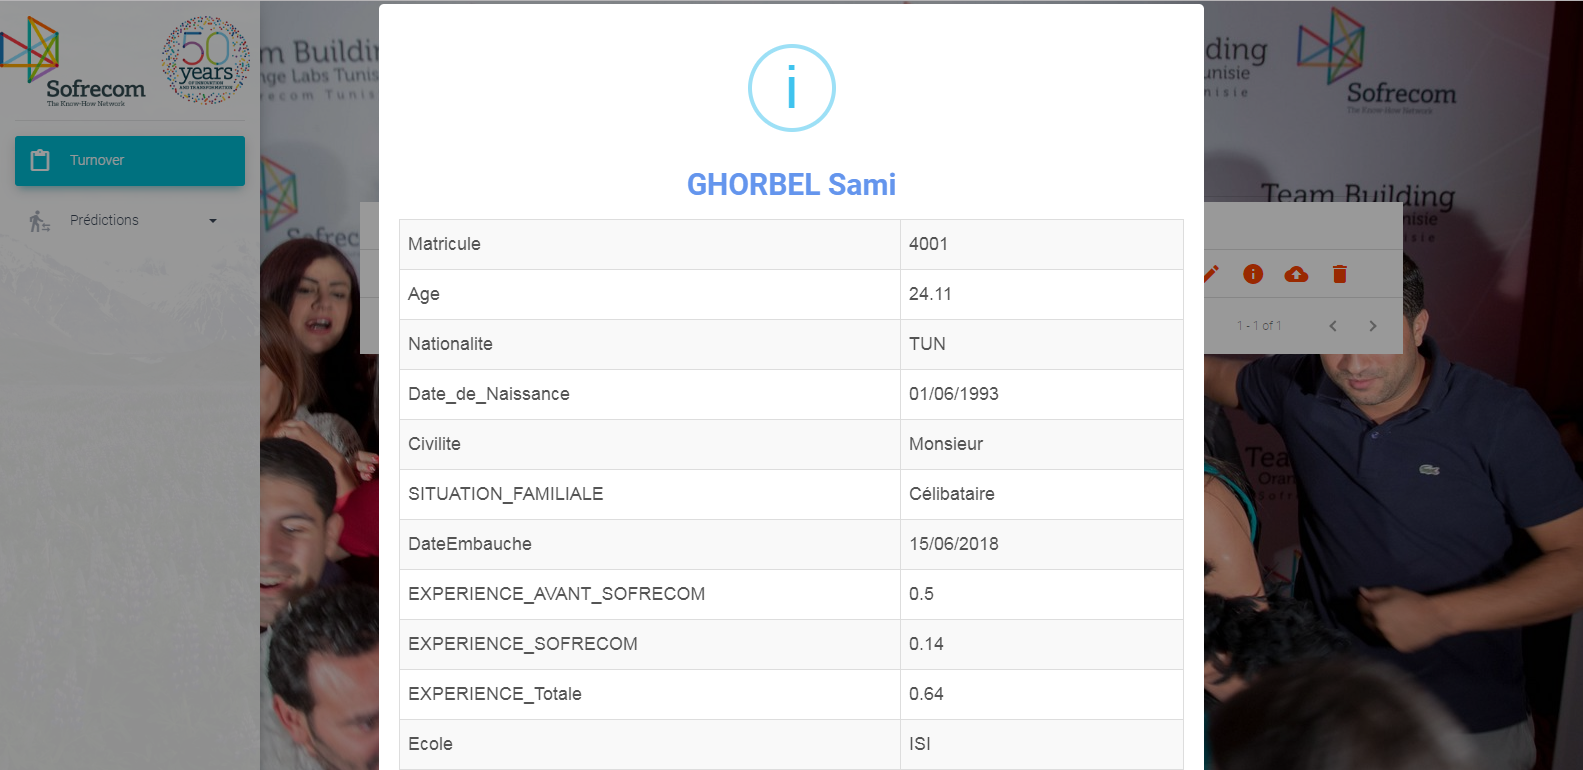
\includegraphics[width=1\linewidth]{img/realisationPFe_sprint2_info.png}}
    \caption{Interface de consultation des informations d'un employé}
    \label{fig:realisationPFe_sprint2_info}
    \end{figure}
\newpage
\textbf{Interface de modification des informations d'un employé}\\
Comme illustré par la figure \ref{fig:realisationPFe_sprint2_modif}, l'utilisateur RH peut modifier les informations d'un employé.

    \begin{figure}[htpb]
    \centering
    \fcolorbox{brown}{white}{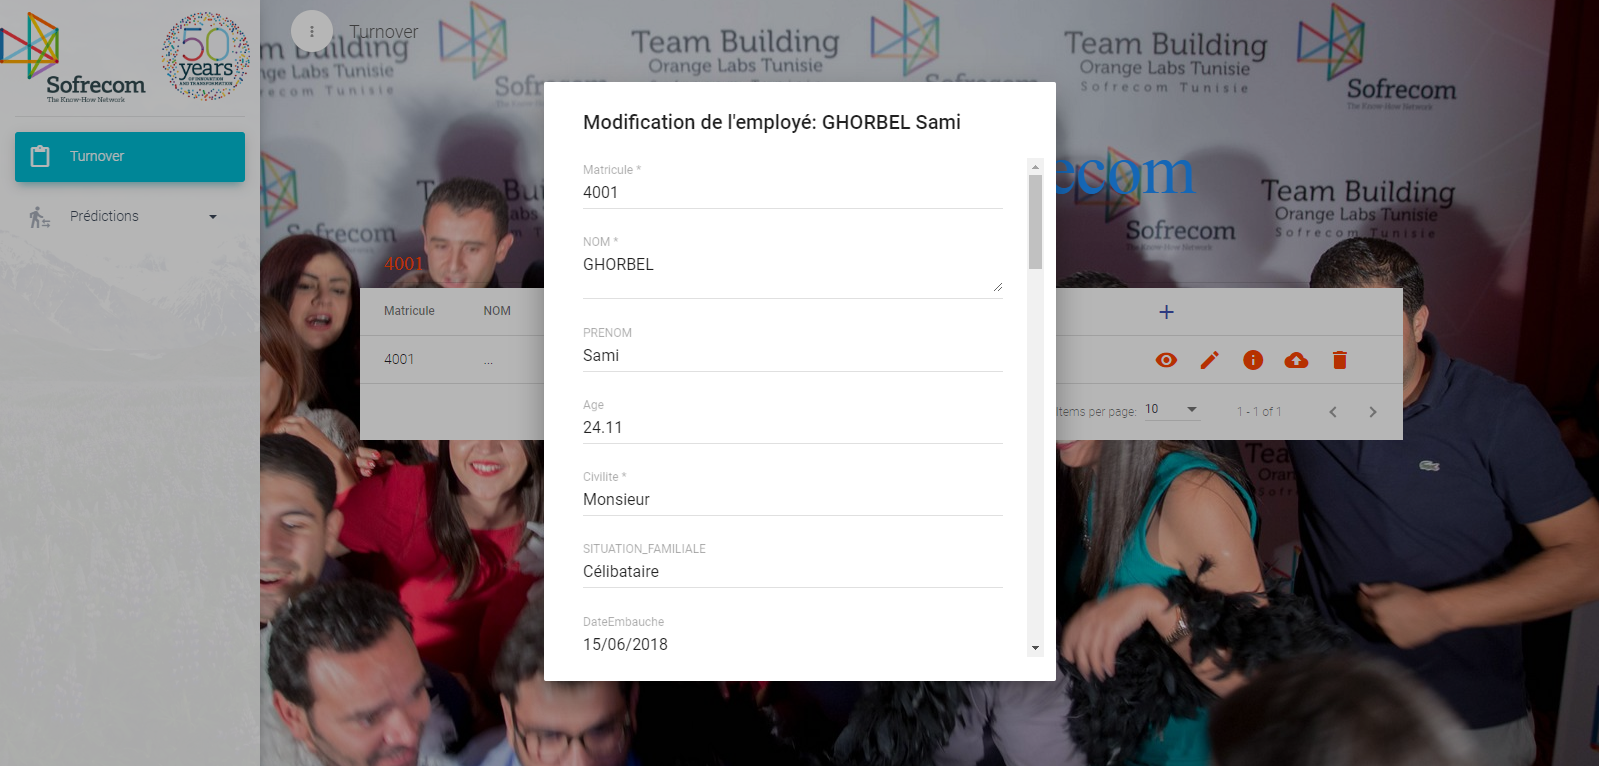
\includegraphics[width=1\linewidth]{img/realisationPFe_sprint2_modif.png}}
    \caption{Interface de modification des informations d'un employé}
    \label{fig:realisationPFe_sprint2_modif}
    \end{figure}
    

\textbf{Interface de confirmation de prédiction d'un employé}\\
Lors de la prédiction, l'utilisateur RH choisit un employé. Une alerte sera déclenchée pour la confirmation de la prédiction sur l'employé concerné comme le montre la figure \ref{fig:realisationPFe_sprint2_confirm_prediction}.
    \begin{figure}[htpb]
    \centering
    \fcolorbox{brown}{white}{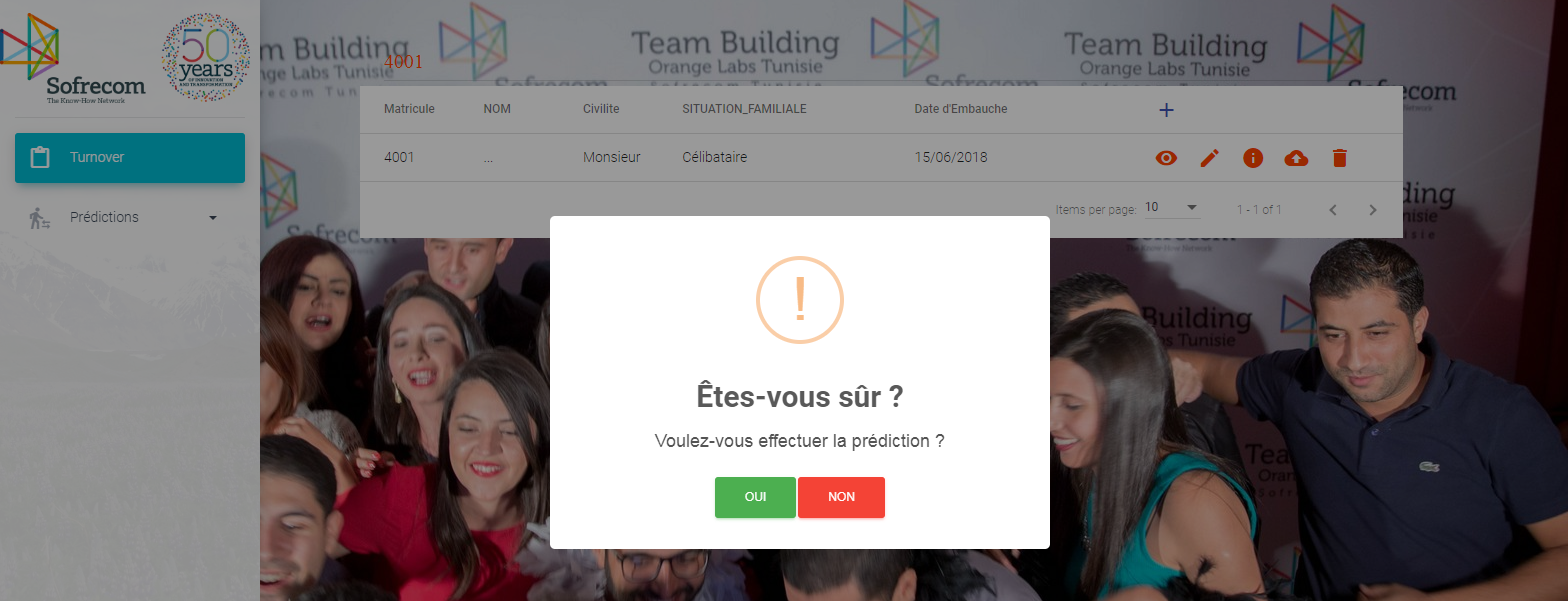
\includegraphics[width=1\linewidth]{img/realisationPFe_sprint2_confirm_prediction.png}}
    \caption{Interface de confirmation de prédiction d'un employé}
    \label{fig:realisationPFe_sprint2_confirm_prediction}
    \end{figure}
    
\newpage

\textbf{Interface de chargement de prédiction d'un employé}\\
Le traitement de prédiction prend un peu de temps pour retourner un résultat. Une alerte de chargement est affichée à l'utilisateur RH comme le montre la figure \ref{fig:realisationPFe_sprint2_prediction}.
    \begin{figure}[htpb]
    \centering
    \fcolorbox{brown}{white}{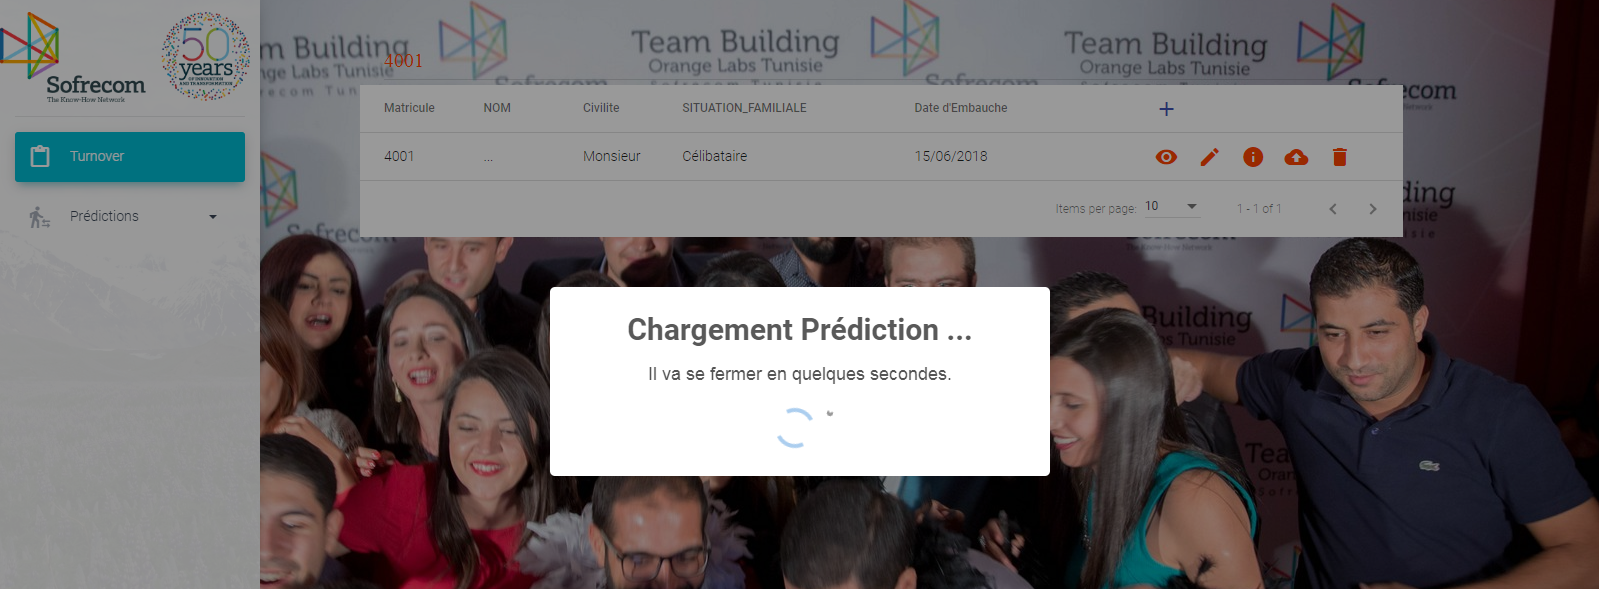
\includegraphics[width=1\linewidth]{img/realisationPFe_sprint2_prediction.png}}
    \caption{Interface de chargement de prédiction d'un employé}
    \label{fig:realisationPFe_sprint2_prediction}
    \end{figure}
    
\textbf{Interface de résultat de prédiction d'un employé}\\
Une fois le traitement de prédiction est terminé, une alerte sera déclenchée pour indiquer le résultat retourné comme illustré sur la figure     \ref{fig:realisationPFe_sprint2_prediction_result}.
    \begin{figure}[htpb]
    \centering
    \fcolorbox{brown}{white}{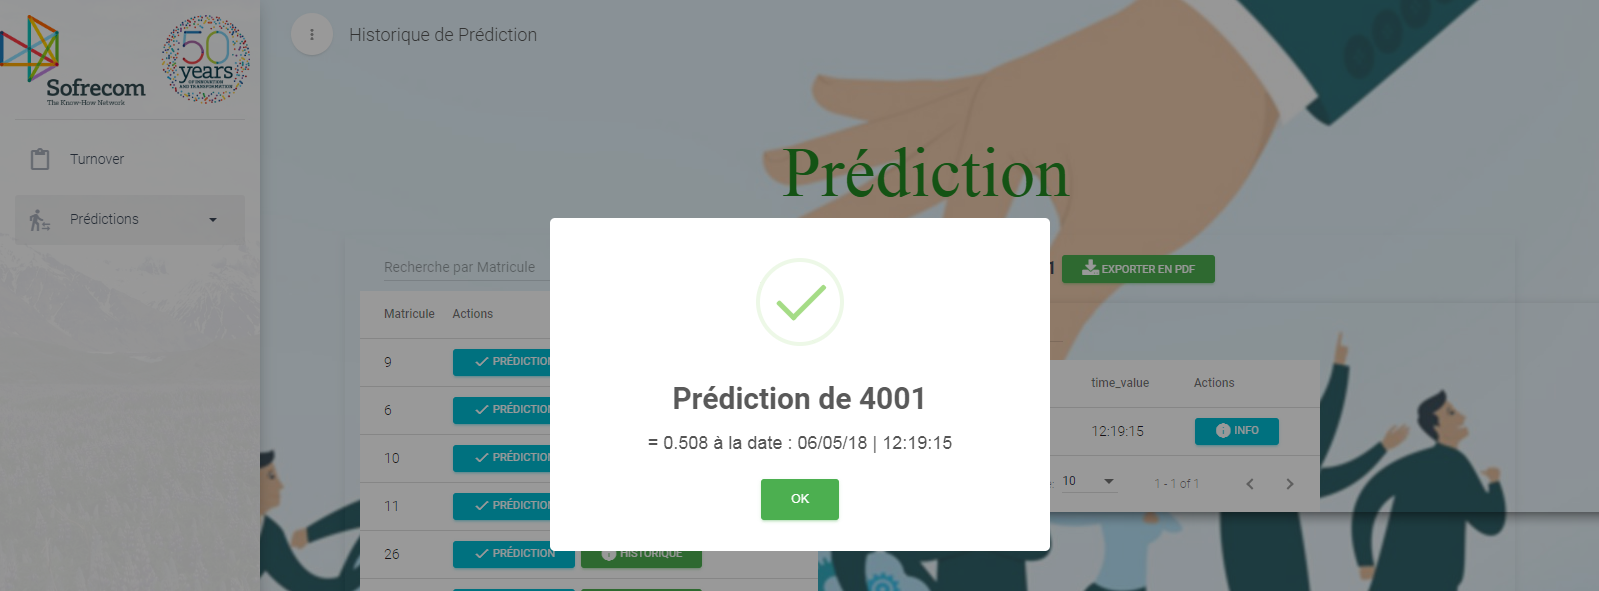
\includegraphics[width=1\linewidth]{img/realisationPFe_sprint2_prediction_result.png}}
    \caption{Interface de résultat de prédiction d'un employé}
    \label{fig:realisationPFe_sprint2_prediction_result}
    \end{figure}

\newpage
\textbf{Interface de suppression d'un employé}\\
L'utilisateur RH choisit un employé à supprimer. Une alerte de confirmation sera déclenchée pour confirmer la suppression de l'employé concerné comme indiqué sur la figure \ref{fig:realisationPFe_sprint2_suppression}.
    \begin{figure}[htpb]
    \centering
    \fcolorbox{brown}{white}{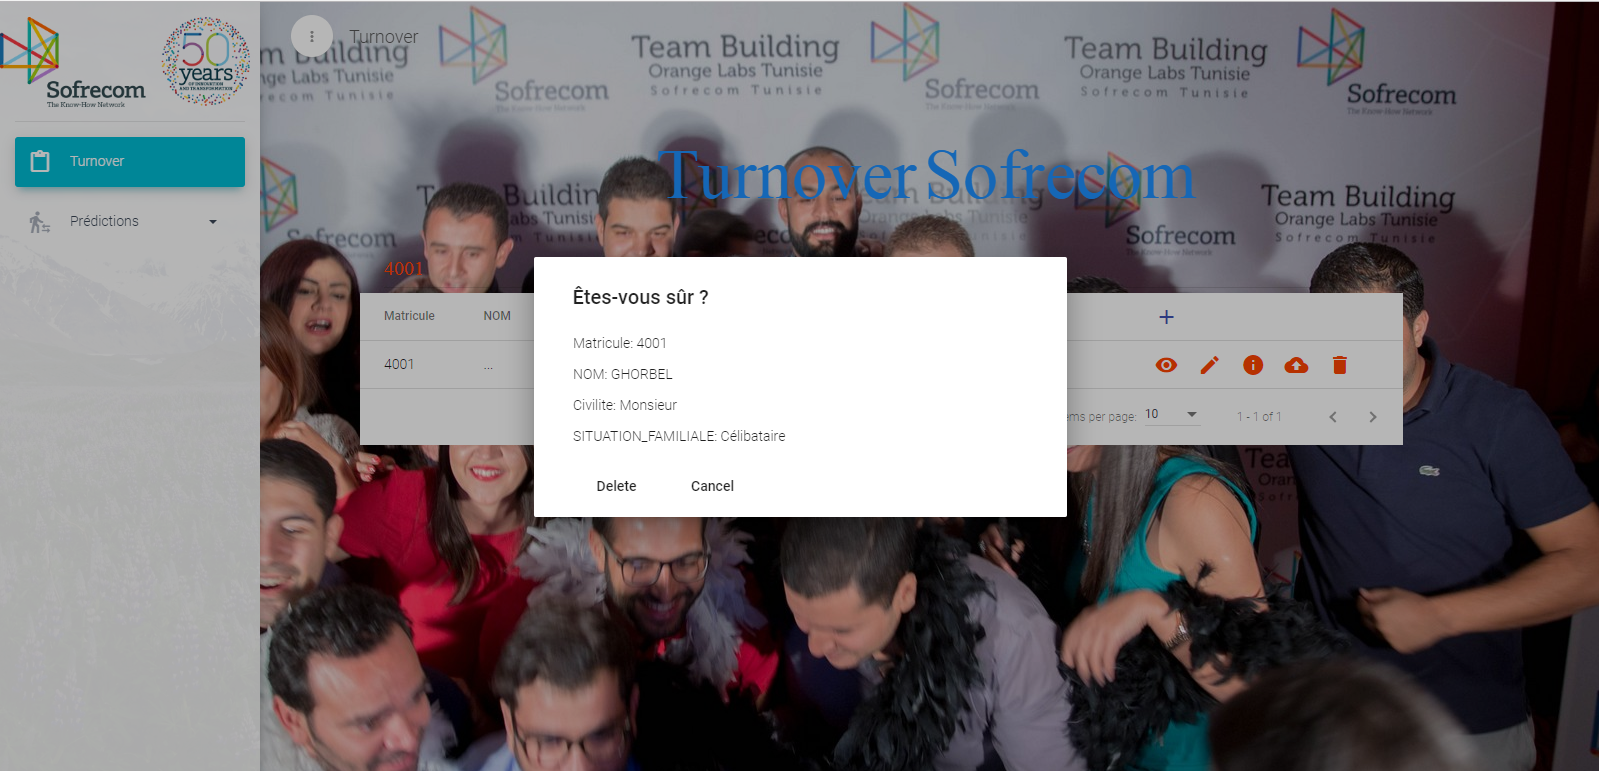
\includegraphics[width=1\linewidth]{img/realisationPFe_sprint2_suppression.png}}
    \caption{Interface de suppression d'un employé}
    \label{fig:realisationPFe_sprint2_suppression}
    \end{figure}


\textbf{Interface de succès de suppression d'un employé}\\
Dès que l'utilisateur RH confirme la suppression de l'employé, une alerte de succès sera affichée comme le montre la figure \ref{fig:realisationPFe_sprint2_suppression2} .
    \begin{figure}[htpb]
    \centering
    \fcolorbox{brown}{white}{\includegraphics[width=1\linewidth]{img/realisationPFe_sprint2_suppression2.png}}
    \caption{Interface de succès de suppression d'un employé}
    \label{fig:realisationPFe_sprint2_suppression2}
    \end{figure}
\newpage

\textbf{Interface de consultation des employés prédits}\\
Comme le montre la figure \ref{fig:realisationPFe_sprint2_prediction_list}, l'utilisateur RH peut consulter la liste des employés dont les prédictions y figurent.
    \begin{figure}[htpb]
    \centering
    \fcolorbox{brown}{white}{\includegraphics[width=1\linewidth]{img/realisationPFe_sprint2_prediction_list.png}}
    \caption{Interface de consultation des employés prédits}
    \label{fig:realisationPFe_sprint2_prediction_list}
    \end{figure}


\textbf{Interface de consultation de l'historique des prédictions d'un employé}\\
L'utilisateur RH peut consulter l'historique des prédictions de chaque employé comme indiqué sur la figure \ref{fig:realisationPFe_sprint2_prediction_histo}.
    \begin{figure}[htpb]
    \centering
    \fcolorbox{brown}{white}{\includegraphics[width=1\linewidth]{img/realisationPFe_sprint2_prediction_histo.png}}
    \caption{Interface de consultation de l'historique des prédictions d'un employé}
    \label{fig:realisationPFe_sprint2_prediction_histo}
    \end{figure}

\newpage

\textbf{Interface d'export de l'historique des informations d'un employé sous format PDF}\\
La figure \ref{fig:realisationPFe_sprint2_prediction_export} représente l’interface permettant à l’utilisateur RH de consulter l'historique des prédictions et des informations d'un employé exporté sous format PDF.


    \begin{figure}[htpb]
    \centering
    \fcolorbox{brown}{white}{\includegraphics[width=1\linewidth]{img/exportpdf.png}}
    \caption{Interface d'export de l'historique des informations d'un employé sous format PDF}
    \label{fig:realisationPFe_sprint2_prediction_export}
    \end{figure}

\subsection{Test et validation}
Nous avons rassemblé dans le tableau 4.11 un ensemble de scénarios de cas de tests fonctionnels associés au sprint 2.
\captionof{table}{Tests fonctionnels du sprint 2}

\begin{tabular}{@{}| p{.25\textwidth}| p{5.1 cm}|p{5.2 cm}| >{\centering\arraybackslash}p{.10\textwidth}|@{}}

\hline \rowcolor{lightgray} \hspace{1.5pc} \textbf{Cas de test}  & \hspace{1.5pc}  \textbf {Démarches} & \hspace{0.5pc}  \textbf {Comportement attendu} &   \textbf {Résultat} \\



\hline  Effectuer une prédiction & Demander la page de gestion des employés.\newline
valider la prédiction d'un employé.
& Affichage de la page de gestion des employés.\newline
Chargement et affichage du résultat de la prédiction.
& Conforme \\




\hline
\end{tabular}


\begin{tabular}{@{}| p{.25\textwidth}| p{5.1 cm}|p{5.2 cm}| >{\centering\arraybackslash}p{.10\textwidth}|@{}}

\hline \rowcolor{lightgray} \hspace{1.5pc} \textbf{Cas de test}  & \hspace{1.5pc}  \textbf {Démarches} & \hspace{0.5pc}  \textbf {Comportement attendu} &   \textbf {Résultat} \\

\hline  Ajouter un employé & Demander la page de gestion des employés.\newline
Cliquer sur ajouter.\newline
Remplir et valider le formulaire d'ajout.
& Affichage de la page de gestion des employés.\newline
Affichage de formulaire d'ajout.\newline
Ajout effectué.


& Conforme \\

\hline  Modifier un employé & Demander la page de gestion des employés.\newline
Cliquer sur modifier.\newline \newline
Saisir et valider le formulaire de modification .
& Affichage de la page de gestion des employés.\newline
Affichage de formulaire de modification.\newline
Modification effectuée.


& Conforme \\


\hline  Supprimer un employé & Demander la page de gestion des employés.\newline
Cliquer sur supprimer.\newline\newline
Confirmer la suppression.
& Affichage de la page de gestion des employés.\newline
Affichage d'un message de confirmation de suppression.\newline
Suppression effectuée.


& Conforme \\

\hline

\end{tabular}
\newline
\newline
  Après avoir vérifié le bon fonctionnement du code et des fonctionnalités, le deuxième livrable a
été testé et validé par le Product Owner. Il est à noter que plusieurs autres tests ont été effectués et conclus à conforme tels que :
\begin{itemize}
    \item consulter la liste des employés predits;
    \item exporter l'historique des prédictions d'un employé;
    \item rechercher un employé prédit;
    \item exporter toutes les informations d'un employé.
\end{itemize}

\section*{Conclusion}

À travers ce chapitre, nous avons réussi à produire un incrément ayant suffisamment de valeur pour
le client et pourra être utilisé dans un environnement de production.
Le chapitre suivant sera consacré pour produire une nouvelle release couvrant les
fonctionnalités d'administration et visualisation.
  